
% \documentclass[a4paper, 12pt, twoside]{article}
% % Language and encoding packages
% \usepackage[T1,T2A]{fontenc} % T2A for cyrillic symbols, T1 for latin symbols
% \usepackage[utf8]{inputenc} % UTF-8 encoding
% \usepackage[russian,english]{babel} % Russian and English languages, where main is English
% % Other packages
% \usepackage{eso-pic} % Add background image
% \usepackage{fancyhdr} % Header and footer settings
% \usepackage{pdfpages} % Include PDF files
% \usepackage{amsmath} % Math package
% %\usepackage{apacite} % APA citation style
% \usepackage[natbibapa]{apacite}
% \usepackage{geometry} % Page geometry
% \geometry{a4paper, margin=1in}

% \usepackage{wrapfig}

% \usepackage{graphicx} % Graphics package for images
% \graphicspath{{./images_thesis/}}

% % Add parskip package for increased paragraph spacing
% \usepackage[skip=10pt]{parskip} % Add parskip package for increased paragraph spacing

% % Add fvextra package for better verbatim environments
% \usepackage{fvextra}
% \fvset{
%   breaklines=true,  % Enable line breaking
%   breakanywhere=true,  % Allow breaks at any character
%   breakautoindent=false,  % No indentation for continued lines
%   tabsize=4  % Set tab size to 4 spaces
%   % make size of the font smaller
%   % fontsize=\small
% }

% % Redefine verbatim environment to use fvextra
% \let\oldverbatim\verbatim
% \let\endoldverbatim\endverbatim
% \renewenvironment{verbatim}{%
%   \VerbatimEnvironment
%   \begin{Verbatim}
% }{%
%   \end{Verbatim}
% }

% % Background image command
% \newcommand\BackgroundPic{%
%     \put(0,0){%
%         \parbox[b][\paperheight]{\paperwidth}{%
%             \vfill
%             \centering
%             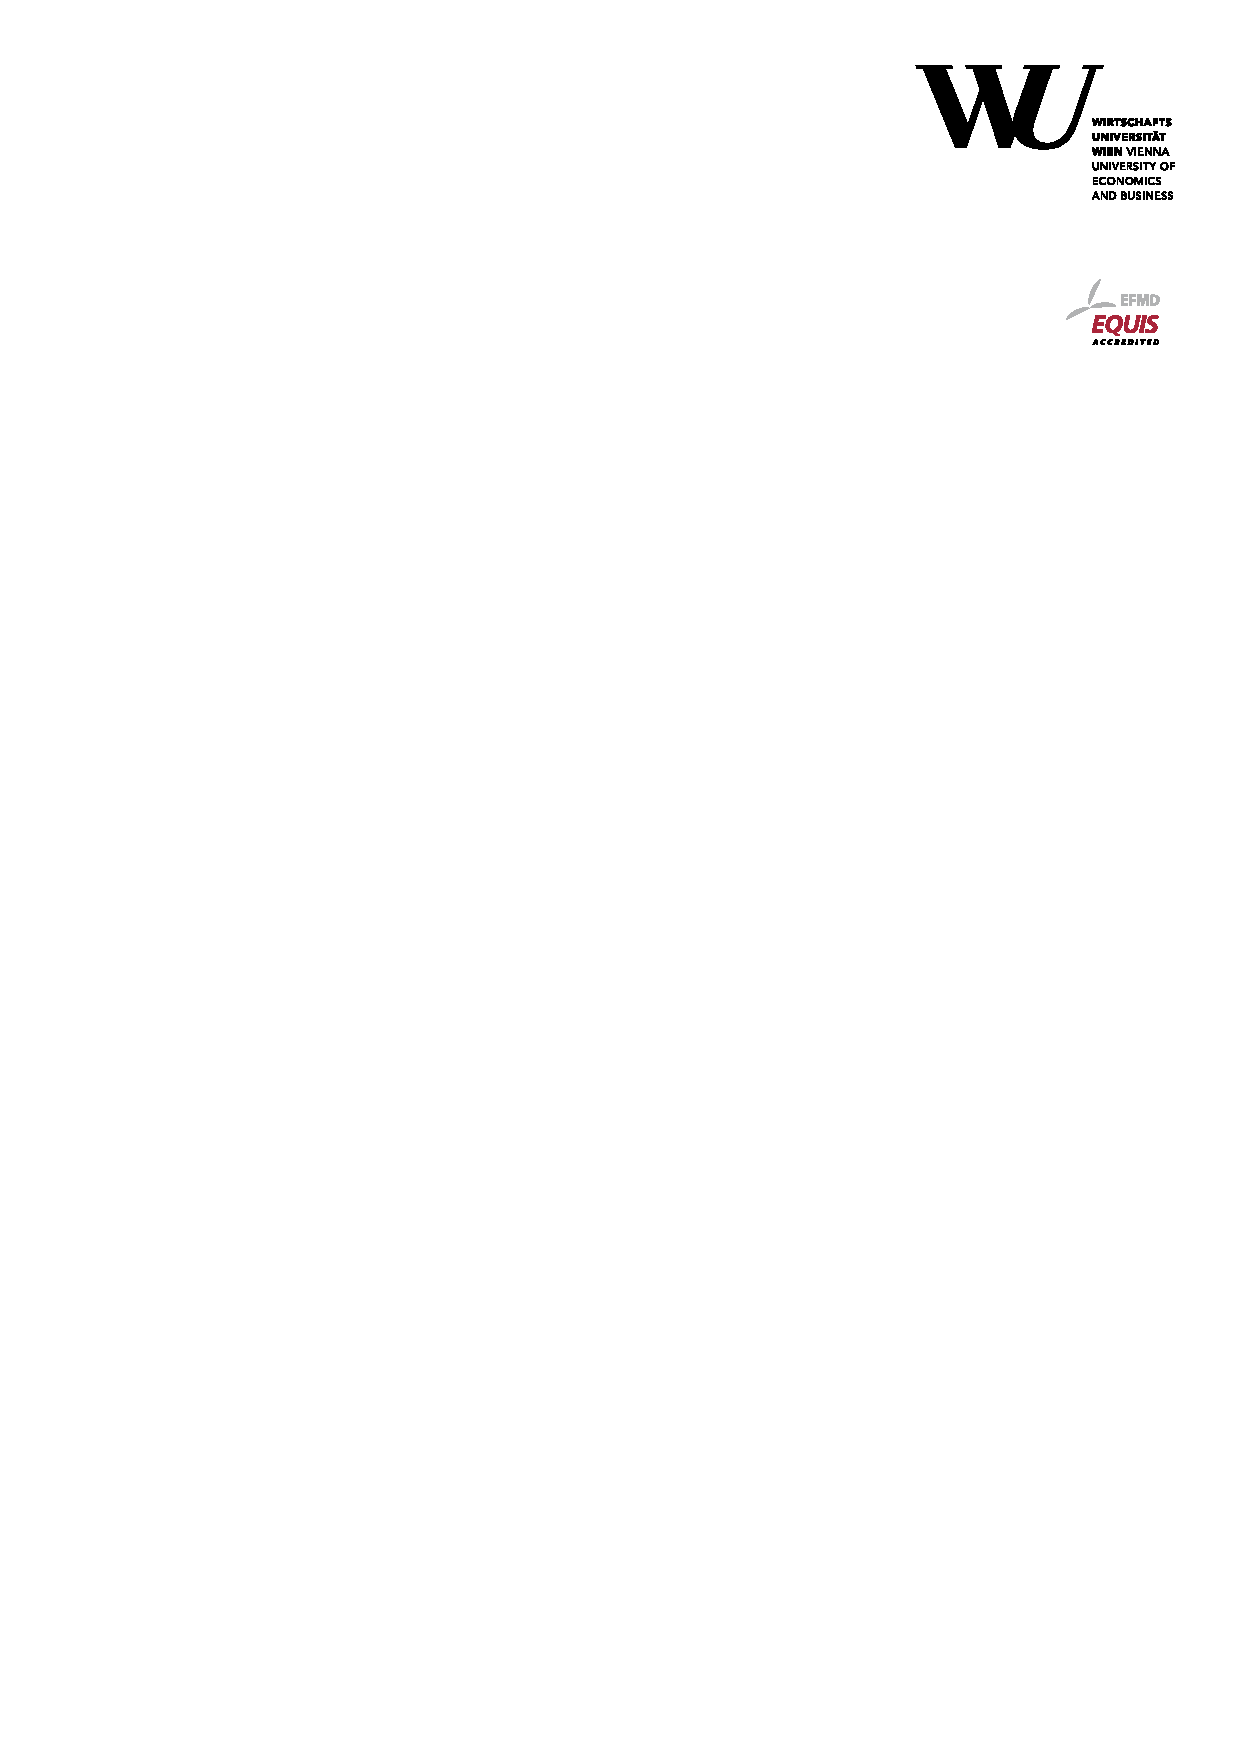
\includegraphics[width=\paperwidth,height=\paperheight,keepaspectratio]{background.pdf}%
%             \vfill
%         }
%     }
% }

% % Add background image to all pages
% \AddToShipoutPictureBG*{\BackgroundPic}
% % Header and footer settings
% \fancyhf{}
% \renewcommand{\headrulewidth}{0pt}
% \renewcommand{\footrulewidth}{0pt}
% \fancyfoot[L]{\hspace*{-16mm}
%     
\includegraphics[scale=0.3]{logoDepartment.pdf}
% }
% \pagestyle{fancy}


% % Place hyperref last to avoid conflicts, where hyperref is used for hyperlinks
% \usepackage{hyperref}

% % add page numbers
% \pagenumbering{arabic}

% \begin{document}

% \AddToShipoutPicture*{\BackgroundPic}
% \thispagestyle{fancy}
% {\vspace{2cm}~}
% {\vspace{2cm}}

% {\noindent\large Bachelor Thesis}
% \vspace{1cm}

% %{\noindent\huge\textbf{Integrating RDF* into the HDT format for efficient management of Wikidata}}
% {\noindent\huge\textbf{RDF Serialisation Using Indexed Predicate Chains}}
% \bigskip

% {\noindent\LARGE Daniil Kovekh}
% \bigskip

% {\noindent\small Date of Birth: 20.04.2002}
% {\noindent\small Student ID: h12014584}
% \bigskip

% {\vspace{2cm}}

% {\noindent\large {\bf Subject Area:} Information Business}
% \bigskip

% {\noindent\large {\bf Studienkennzahl:} Bachelor in Business and Economics}
% \bigskip

% {\noindent\large {\bf Supervisor:} Amin Anjomshoaa}
% \bigskip

% {\noindent\large {\bf Date of Submission:} 15.09.2024}
% \bigskip\bigskip\bigskip\bigskip\bigskip\bigskip

% {\em\noindent Department of Information Systems \& Operations Management, Vienna University of
% Economics and Business, Welthandelsplatz 1, 1020 Vienna, Austria
% }
% \pagebreak

% \tableofcontents

% \clearpage  % This ensures the abstract starts on a new page

\documentclass[a4paper, 12pt, twoside]{article}

%------------------------------------------------
% Language and Encoding Packages
%------------------------------------------------
\usepackage[T1,T2A]{fontenc}        % T2A for Cyrillic symbols, T1 for Latin symbols
\usepackage[utf8]{inputenc}         % UTF-8 encoding
\usepackage[russian,english]{babel} % Russian and English languages, main is English

%------------------------------------------------
% Geometry and Layout
%------------------------------------------------
\usepackage{geometry}               % Page geometry
\geometry{a4paper, margin=1in}

%------------------------------------------------
% Graphics and Images
%------------------------------------------------
\usepackage{graphicx}               % Graphics package for images
\graphicspath{{./images_thesis/}}   % Path to images directory

%------------------------------------------------
% Header and Footer Settings
%------------------------------------------------
\usepackage{fancyhdr}               % Header and footer settings
\usepackage{eso-pic}                % Add background image

%------------------------------------------------
% Other Essential Packages
%------------------------------------------------
\usepackage{amsmath}                % Math package
\usepackage{pdfpages}               % Include PDF files
\usepackage[natbibapa]{apacite}     % APA citation style
\usepackage{wrapfig}                % Wrap figures
\usepackage[skip=10pt]{parskip}     % Increased paragraph spacing

%------------------------------------------------
% Verbatim Environment Enhancement
%------------------------------------------------
\usepackage{fvextra}                % Better verbatim environments
\fvset{
  breaklines=true,                  % Enable line breaking
  breakanywhere=true,                % Allow breaks at any character
  breakautoindent=false,             % No indentation for continued lines
  tabsize=4                          % Set tab size to 4 spaces
}

% Redefine verbatim environment to use fvextra
\let\oldverbatim\verbatim
\let\endoldverbatim\endverbatim
\renewenvironment{verbatim}{%
  \VerbatimEnvironment
  \begin{Verbatim}
}{%
  \end{Verbatim}
}

%------------------------------------------------
% Background Image Configuration
%------------------------------------------------
\newcommand\BackgroundPic{%
    \put(0,0){%
        \parbox[b][\paperheight]{\paperwidth}{%
            \vfill
            \centering
            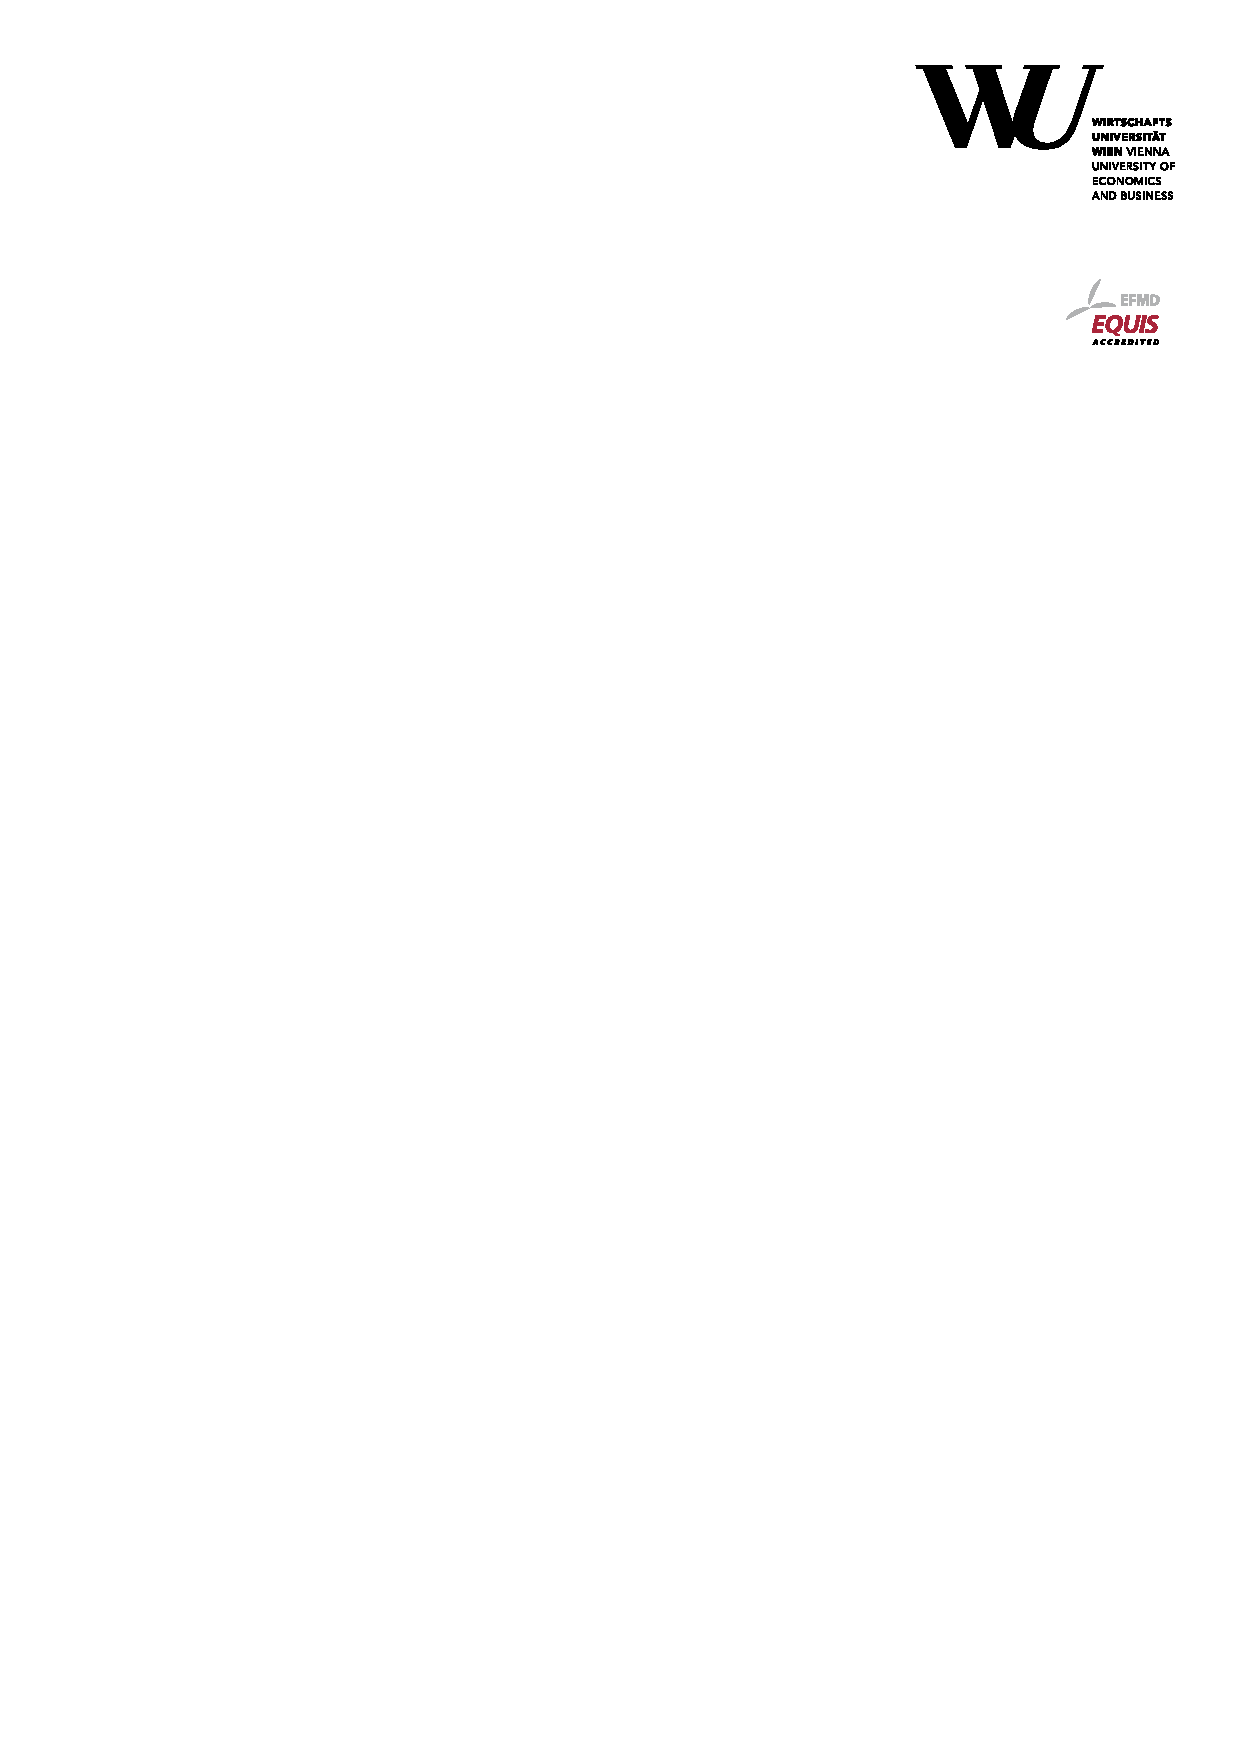
\includegraphics[width=\paperwidth,height=\paperheight,keepaspectratio]{background.pdf}%
            \vfill
        }
    }
}

% Add background image to all pages
\AddToShipoutPictureBG*{\BackgroundPic}

%------------------------------------------------
% Fancyhdr Configuration for Headers and Footers
%------------------------------------------------
\fancyhf{} % Clear all header and footer fields

% Add the department logo to the left side of the footer
\fancyfoot[L]{%
    \hspace*{-16mm}
    
\includegraphics[scale=0.3]{logoDepartment.pdf}
}

% Add page numbers to the center of the footer
\fancyfoot[C]{\thepage}

% Remove header and footer lines
\renewcommand{\headrulewidth}{0pt}
\renewcommand{\footrulewidth}{0pt}

% Apply the fancy page style
\pagestyle{fancy}

%------------------------------------------------
% Hyperref Package (Place Last to Avoid Conflicts)
%------------------------------------------------
\usepackage{hyperref}

%------------------------------------------------
% Page Numbering
%------------------------------------------------
\pagenumbering{arabic} % Start page numbering in Arabic numerals

%------------------------------------------------
% Document Content
%------------------------------------------------
\begin{document}

%------------------------------------------------
% Title Page
%------------------------------------------------
\AddToShipoutPicture*{\BackgroundPic} % Ensure background on title page
\thispagestyle{empty}                % Remove page number from title page

\vspace*{2cm} % Top margin for the title page

%------------------------------------------------
% Title Information
%------------------------------------------------
\noindent\large Bachelor Thesis
\vspace{1cm}

\noindent\huge\textbf{RDF Serialisation Using Indexed Predicate Chains}
\bigskip

\noindent\LARGE Daniil Kovekh
\bigskip

\noindent\small Date of Birth: 20.04.2002 \\
\noindent\small Student ID: h12014584
\bigskip

\vspace{2cm}

\noindent\large \textbf{Subject Area:} Information Business
\bigskip

\noindent\large \textbf{Studienkennzahl:} Bachelor in Business and Economics
\bigskip

\noindent\large \textbf{Supervisor:} Dr. Amin Anjomshoaa
\bigskip

\noindent\large \textbf{Date of Submission:} 16.09.2024
\bigskip\bigskip\bigskip\bigskip\bigskip\bigskip

\noindent Department of Information Systems \& Operations Management, Vienna University of Economics and Business, Welthandelsplatz 1, 1020 Vienna, Austria

\pagebreak

%------------------------------------------------
% Table of Contents
%------------------------------------------------
% \tableofcontents
{\small
\tableofcontents
}
\clearpage

%------------------------------------------------
% Abstract
%------------------------------------------------
\begin{abstract}
    The rapid growth of large-scale linked data, such as Wikidata, has necessitated the development of efficient methods for managing and querying Resource Description Framework (RDF) data. 

    RDF* was introduced as an extension to RDF, allowing triples to be treated as subjects and receiving description of itself. However, RDF* has drawbacks, such as increased data complexity and inefficient storage and querying, particularly for large-scale knowledge bases.
    
    Our research identifies three key challenges in RDF* data management: inefficient serialization of RDF*, storage overhead of qualified statements, and inadequate representation of temporal and repeated relationships. To address these issues, we propose a new serialisation format of RDF, that includes chains of predicates and indexed values, eliminating intermediary statement nodes (e.g., statement qualifiers) while preserving context and provenance information.
    
    This thesis addresses two primary research questions: Can RDF Star (RDF*) be effectively integrated into the Header-Dictionary-Triples (HDT) format for improved Wikidata management, and is it possible to develop a more efficient format that retains RDF* properties while leveraging HDT's compression capabilities?
    
    We demonstrate our effectiveness of approach via experiments on a Wikidata subset, comparing it with traditional RDF and HDT representations. Our results show improved efficiency in handling repetitive data, improved readability, and a clear structure that simplifies data hierarchy interpretation.
    
    The new format offers a more efficient and expressive way to represent complex, metadata-rich RDF data, particularly ones, having multiple layers of references to other statemnts. 

    % The challenge, therefore, is to develop a method that can leverage the expressive power of RDF* while avoiding the pitfalls of increased complexity and redundancy. 
\end{abstract}

\clearpage 

\section{Introduction}

In today's digital world, we witness an unprecedented explosion of data. Organizations across the globe are grappling with vast amounts of information spread across numerous databases, catalogs, and reports. This fragmentation of data poses a significant challenge: how to see the big picture of data and how make data-driven decisions quickly? Knowledge graphs, which are one of the existing approaches to address data fragmentation challenges, offer a powerful solution. A Knowledge Graph uses a graph-based model to represent real-world entities, their attributes, and relationships. Entities are anything that can be uniquely identified and described, such as people, places, things, or concepts, and relationships between them \citep{HoganRDF}.

Linked data is a method of publishing structured data in formats like subject, property, object. This data can be interlinked and become more useful through semantic queries, especially if the linked data has a huge number of connections. Imagine a pharmaceutical company, linking data about chemical compounds, clinical trials, and patient data. This interconnected approach allows for more comprehensive insights and discoveries \citep{bizer2011linkeddata}. Moreover, knowledge graphs represent a network of real-world entities – people, places, events – and illustrate how entities are related to each another \citep{ehrlinger2016towards}.

One of the primary advantages of linked data and knowledge graphs is their ability to integrate diverse data sources. Consider a retail bank: it could link customer transaction data, credit scores, social media activity, and market trends into a unified knowledge graph. Probably, some parameters would be irrelevant to each each other, but some can relate to each other significantly, which would not be obvious in a structured database. This comprehensive view allows the bank to offer personalized financial advice, detect fraudulent activities more effectively, and identify cross-selling opportunities. For example, if the graph shows a customer has recently purchased a home, the bank might offer them a competitive home insurance policy \citep{singhal2012introducing}.

Moreover, linked data and knowledge graphs enhance data transparency. For example, government tax offices, can use linked data to identify fraudulent activities. They visualize all transactions and connections between operations, then abnormal situations become more apparent, making it easier to detect potential bribes or other illegal activities.

The applications of these technologies extend far beyond finance and governance. In healthcare, linked data and knowledge graphs are revolutionizing patient care and medical research. By connecting patient records, genetic data, research papers, and clinical trial results, doctors can make more informed decisions. For instance, when treating a patient with a rare disease, a doctor can look at the knowledge graph (or some specific app, that makes additional assumptions), that links symptoms, potential treatments, and outcomes from similar cases that are in this database and may include worldwide history. This interconnected approach might reveal treatment options that wouldn't be feasible when looking at the patient's data in isolation.

As we delve deeper into the world of linked data and knowledge graphs, we encounter a fundamental technology that underpins many of these systems: the Resource Description Framework (RDF). RDF provides a standard model for data interchange on the Web, with well-defined concepts and abstract syntax \citep{cyganiak2014rdf}. It offers express statements about resources in the form of triples: subject, predicate, and object \citep{fernandez2018hdtq}. This structure allows for the representation of complex networks of information, where entities can be interconnected through various relationships.

In a growth of large-scale knowledge bases like Wikidata, we face new challenges in storing, querying, and managing information. The traditional approaches become less relevant due to constraints and rules used in in the data models, like statements in Wikidata.

Our research is guided by two primary questions: Can RDF Star (RDF*) be effectively integrated into the Header-Dictionary-Triples (HDT) format to improve the management of Wikidata-like datasets? This question arises from the need to combine the expressive power of RDF* with the compression efficiency of HDT. RDF* allows for more nuanced metadata representation by treating triples as subjects, which is particularly useful for representing complex statements in Wikidata. However, this added expressiveness often comes at the cost of increased storage requirements and query complexity. By exploring the integration of RDF* with HDT, we aim to determine if it's possible to maintain the benefits of both technologies while mitigating their individual limitations.

The second research question is, whether it possible to develop a more efficient format that retains RDF* properties while leveraging HDT's compression capabilities? Building on the first question, we investigate into finding a possible solution, that captures the power of RDF* while achieving the storage efficiency of HDT. This involves rethinking how we represent RDF data, particularly for large-scale knowledge bases like Wikidata.

In the following chapters, we will delve into the technical details of RDF, explore current storage techniques and their limitations, and propose a our approach.

\subsection{RDF Fundamentals}

As we dive deeper into the linked data and knowledge graphs, it's crucial to understand the building blocks of Resource Description Framework (RDF) – triples and their consistence and to learn about RDF itself. RDF a standard model for data interchange on the Web, with well-defined concepts and abstract syntax \citep{cyganiak2014rdf}. In this section, we'll explore RDF, its extension RDF*, and a powerful format for storing RDF data called HDT.

\subsubsection{Resource Description Framework (RDF)}

Imagine describing the world around you in a way that both humans and machines can understand. RDF does that for data. RDF provides a simple way to express statements about resources in the form of triples: subject, predicate, and object. The predicate is a node that connects the subject with an object.

For instance, to represent the fact that Albert Einstein was born in Germany, we write the following statement: <Einstein> <Country of birth> <Germany>. We call such statement a triple.
Here, "Einstein" is a subject, "Country of birth" is a predicate, and "Germany" is an object. This simple structure allows building complex networks of information, where entities (like Albert Einstein) can be connected to other object through various relationships.

\begin{figure}[htbp]
    \centering
    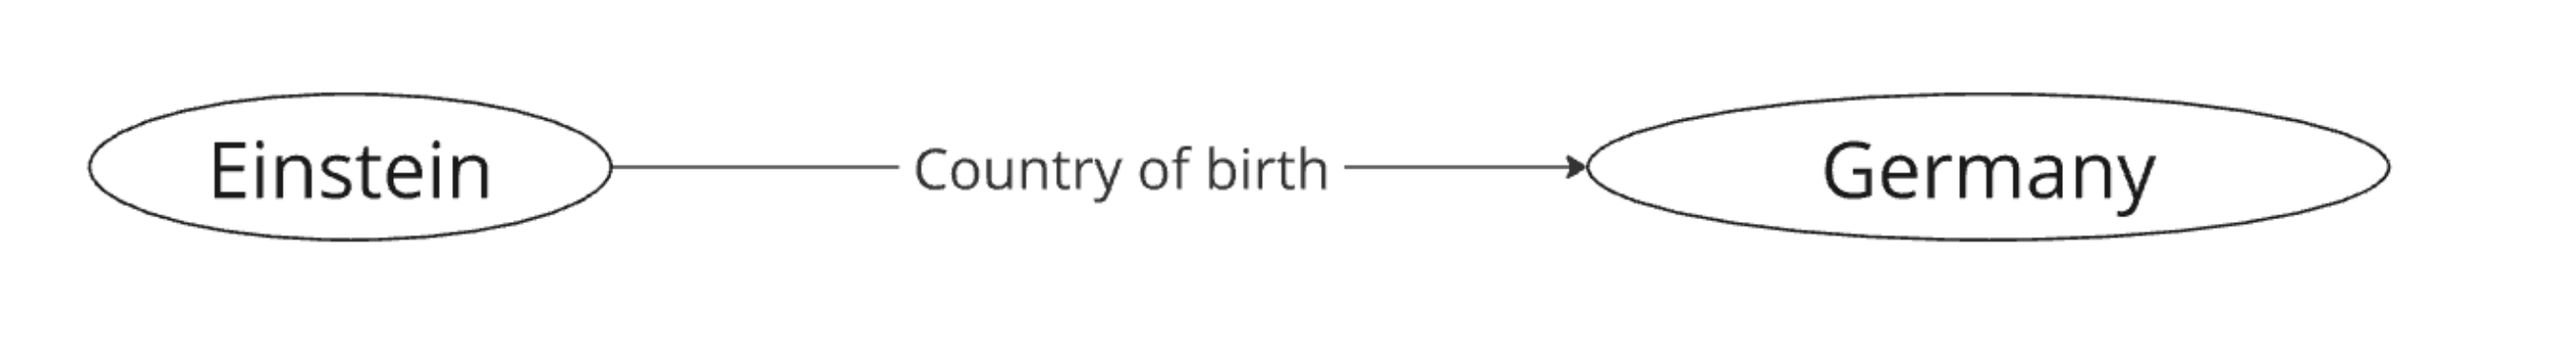
\includegraphics[width=0.8\textwidth]{1.png}
    \caption{simple RDF triple}
    \label{fig:image1}
\end{figure}

RDF is not limited to just connecting entities. The objects may also be literals: strings, integers, floating-point numbers, booleans, dates and times and some custom data types \citep{cyganiak2014rdf}:. For example, "Albert Einstein", "Albert Einstein"@en or \texttt{"1879"{\textasciicircum}{\textasciicircum}xsd:integer}. Objects can be IRIs (Internationalized Resource Identifiers), which are unique identifiers similar to URIs, such as http://dbpedia.org/resource/Germany for Germany \citep{cyganiak2014rdf}. It can also be a blank node - Anonymous resource without global identifier \citep{cyganiak2014rdf}. The values are written in such form:

\begin{figure}[htbp]
    \centering
    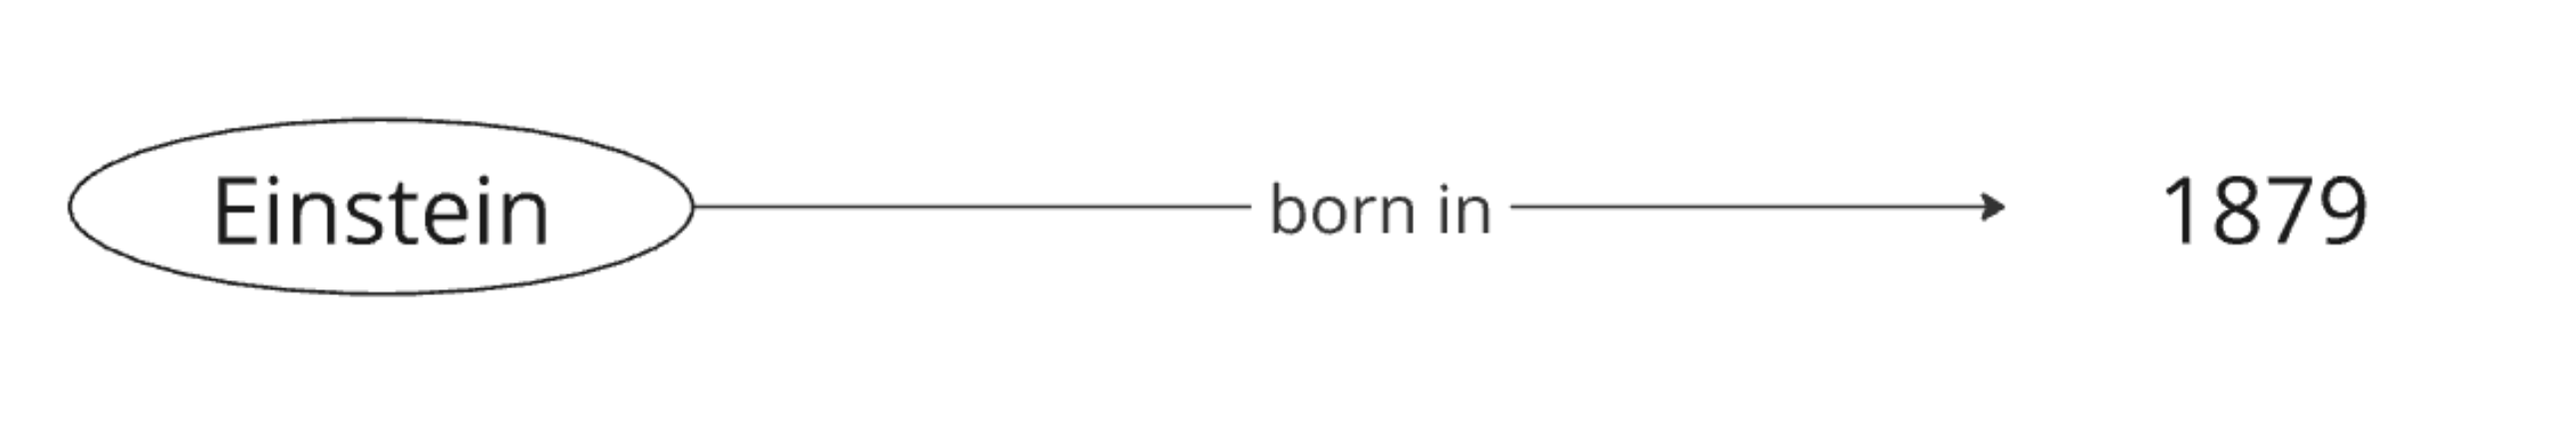
\includegraphics[width=0.8\textwidth]{2.png}
    \caption{simple RDF triple with literal object}
    \label{fig:image2}
\end{figure}

{\footnotesize
\begin{verbatim}
<Albert_Einstein> <born in> "1879"^^xsd:integer.
\end{verbatim}
}

The objects can also be subjects and subjects can be objects as well. However, the subject must be either an IRI or a blank node. The predicate must be an IRI and the object can be either an IRI, a blank node or a literal. This restriction exists because RDF is designed to make statements about resources, and literals are not considered resources in this context. However, it is possible to use Reification – creating a new resource to represent a statement about the literal. Some extensions also allow to represent subjects as literals (OWL), or as triples (RDF*). In the research I use generalised RDF triples, including objects, that may be IRI, blank nodes or literals \citep{cyganiak2014rdf}.

\begin{figure}[htbp]
    \centering
    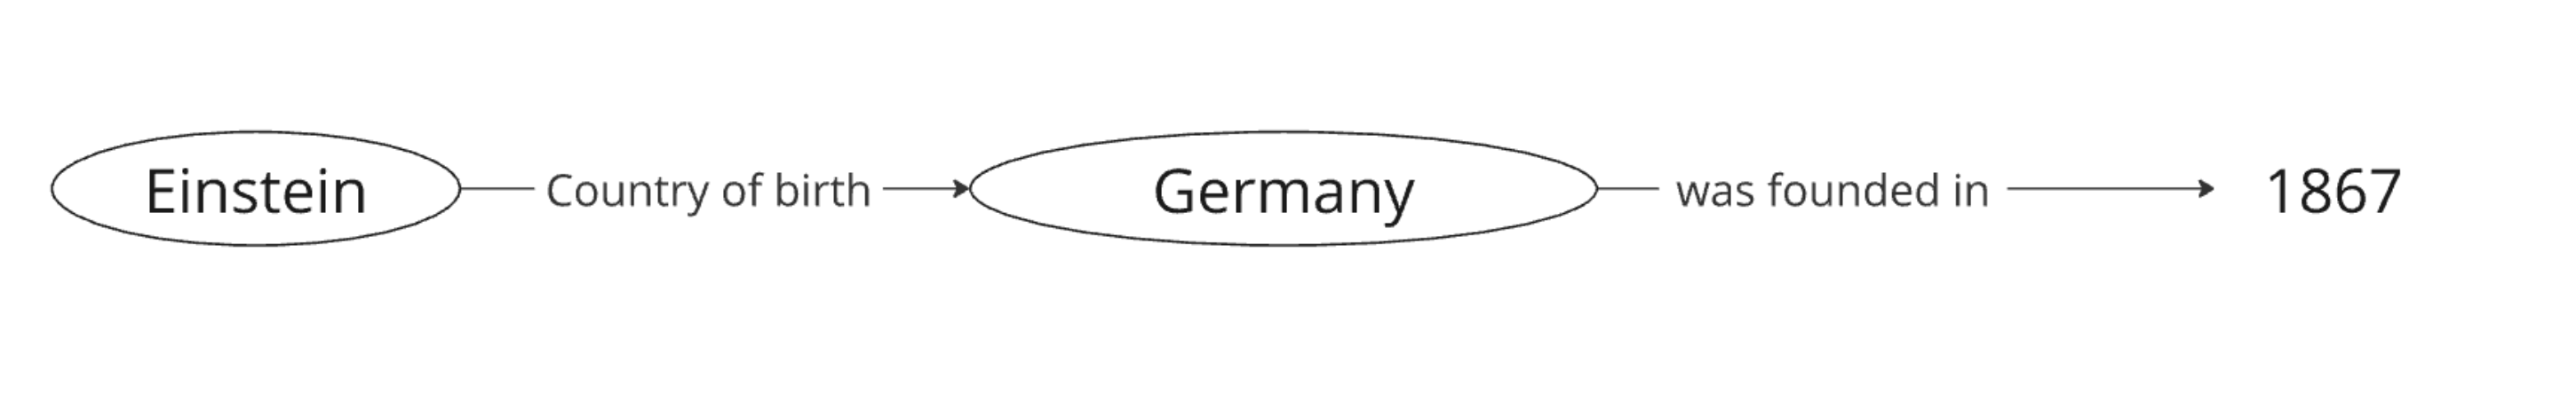
\includegraphics[width=0.8\textwidth]{3.png}
    \caption{multiple RDF triples, with IRI as object and subject}
    \label{fig:image3}
\end{figure}

This flexibility allows RDF to represent a wide range of information, from simple facts to complex relationships between entities. The interesting things start when there is more than one subject and when subjects have something in common.

\begin{figure}[htbp]
    \centering
    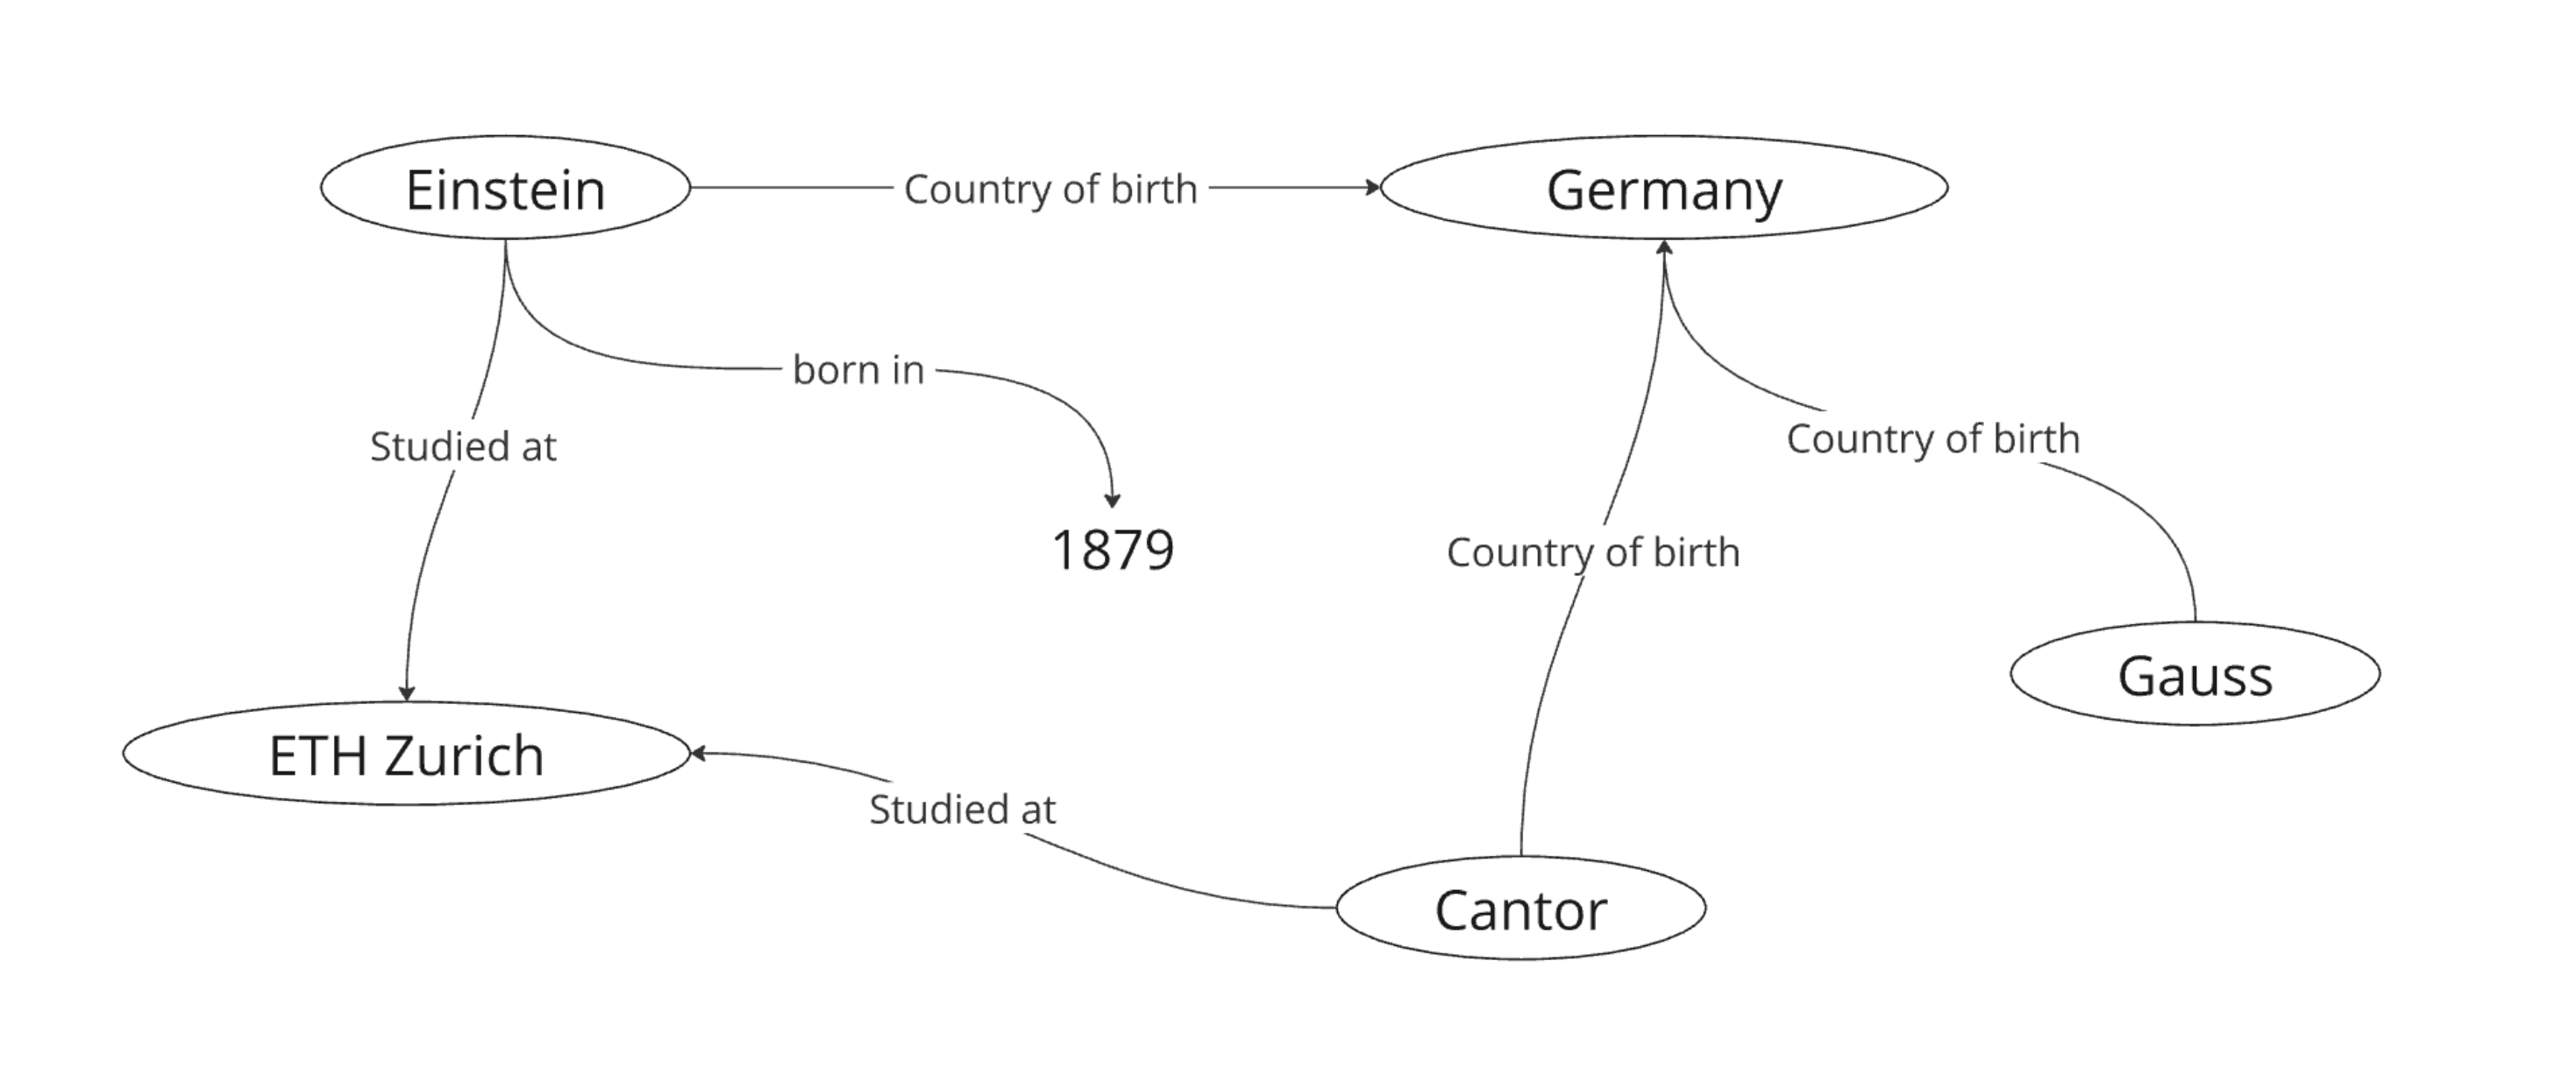
\includegraphics[width=0.8\textwidth]{4.png}
    \caption{multiple RDF triples, with multiple subjects and objects}
    \label{fig:image4}
\end{figure}

In this example, multiple triples and subjects are interconnected in a graph structure. By examining this graph, we can easily see that Einstein and Cantor shared both a university and country of birth. This simple representation allows us to quickly identify connections that might not be immediately apparent when looking at isolated facts. Now, imagine scaling this concept to a massive graph with billions of entities (subjects and objects). Such a structure would allow us to uncover important, high-value information, from identifying all alumni of a particular institution to tracing Einstein's academic lineage – his fellow students, his own students, and those who built upon his research. Applying this concept to the corporate world opens up even more possibilities. For instance, in a large multinational corporation, we could map out complex organizational structures, tracking employees' work history, project contributions, skill sets, and professional relationships.

\subsubsection{RDF Serialisation Formats}

There are multiple serialisation formatss of RDF, each of them having specific functionality. Two most popular formats are Turtle and N-Triples. Wikidata and other popular databases, like Openfoodfacts \citep{openfoodfacts} offer serialisations in those formats. There are also libraries for C++, Java and Python to serialise and work with these formats. 

% Parsing into memory takes some time. Based on insights from different discussions, the common guideline is to allocate around 10GB of RAM for every billion triples. 1 billion triples is approximately 5GB of data \citep{openlinkSoftware}.

Another format is HDT – Headers, Dictionary, Triples – which is an RDF representation in the form of structured data, where subjects, predicates and objects are assigned in the dictionary to a unique identifier, and are written in a Triple section in a form of unique identifier to save space by not repeating similar arguments.

\begin{figure}[htbp]
    \centering
    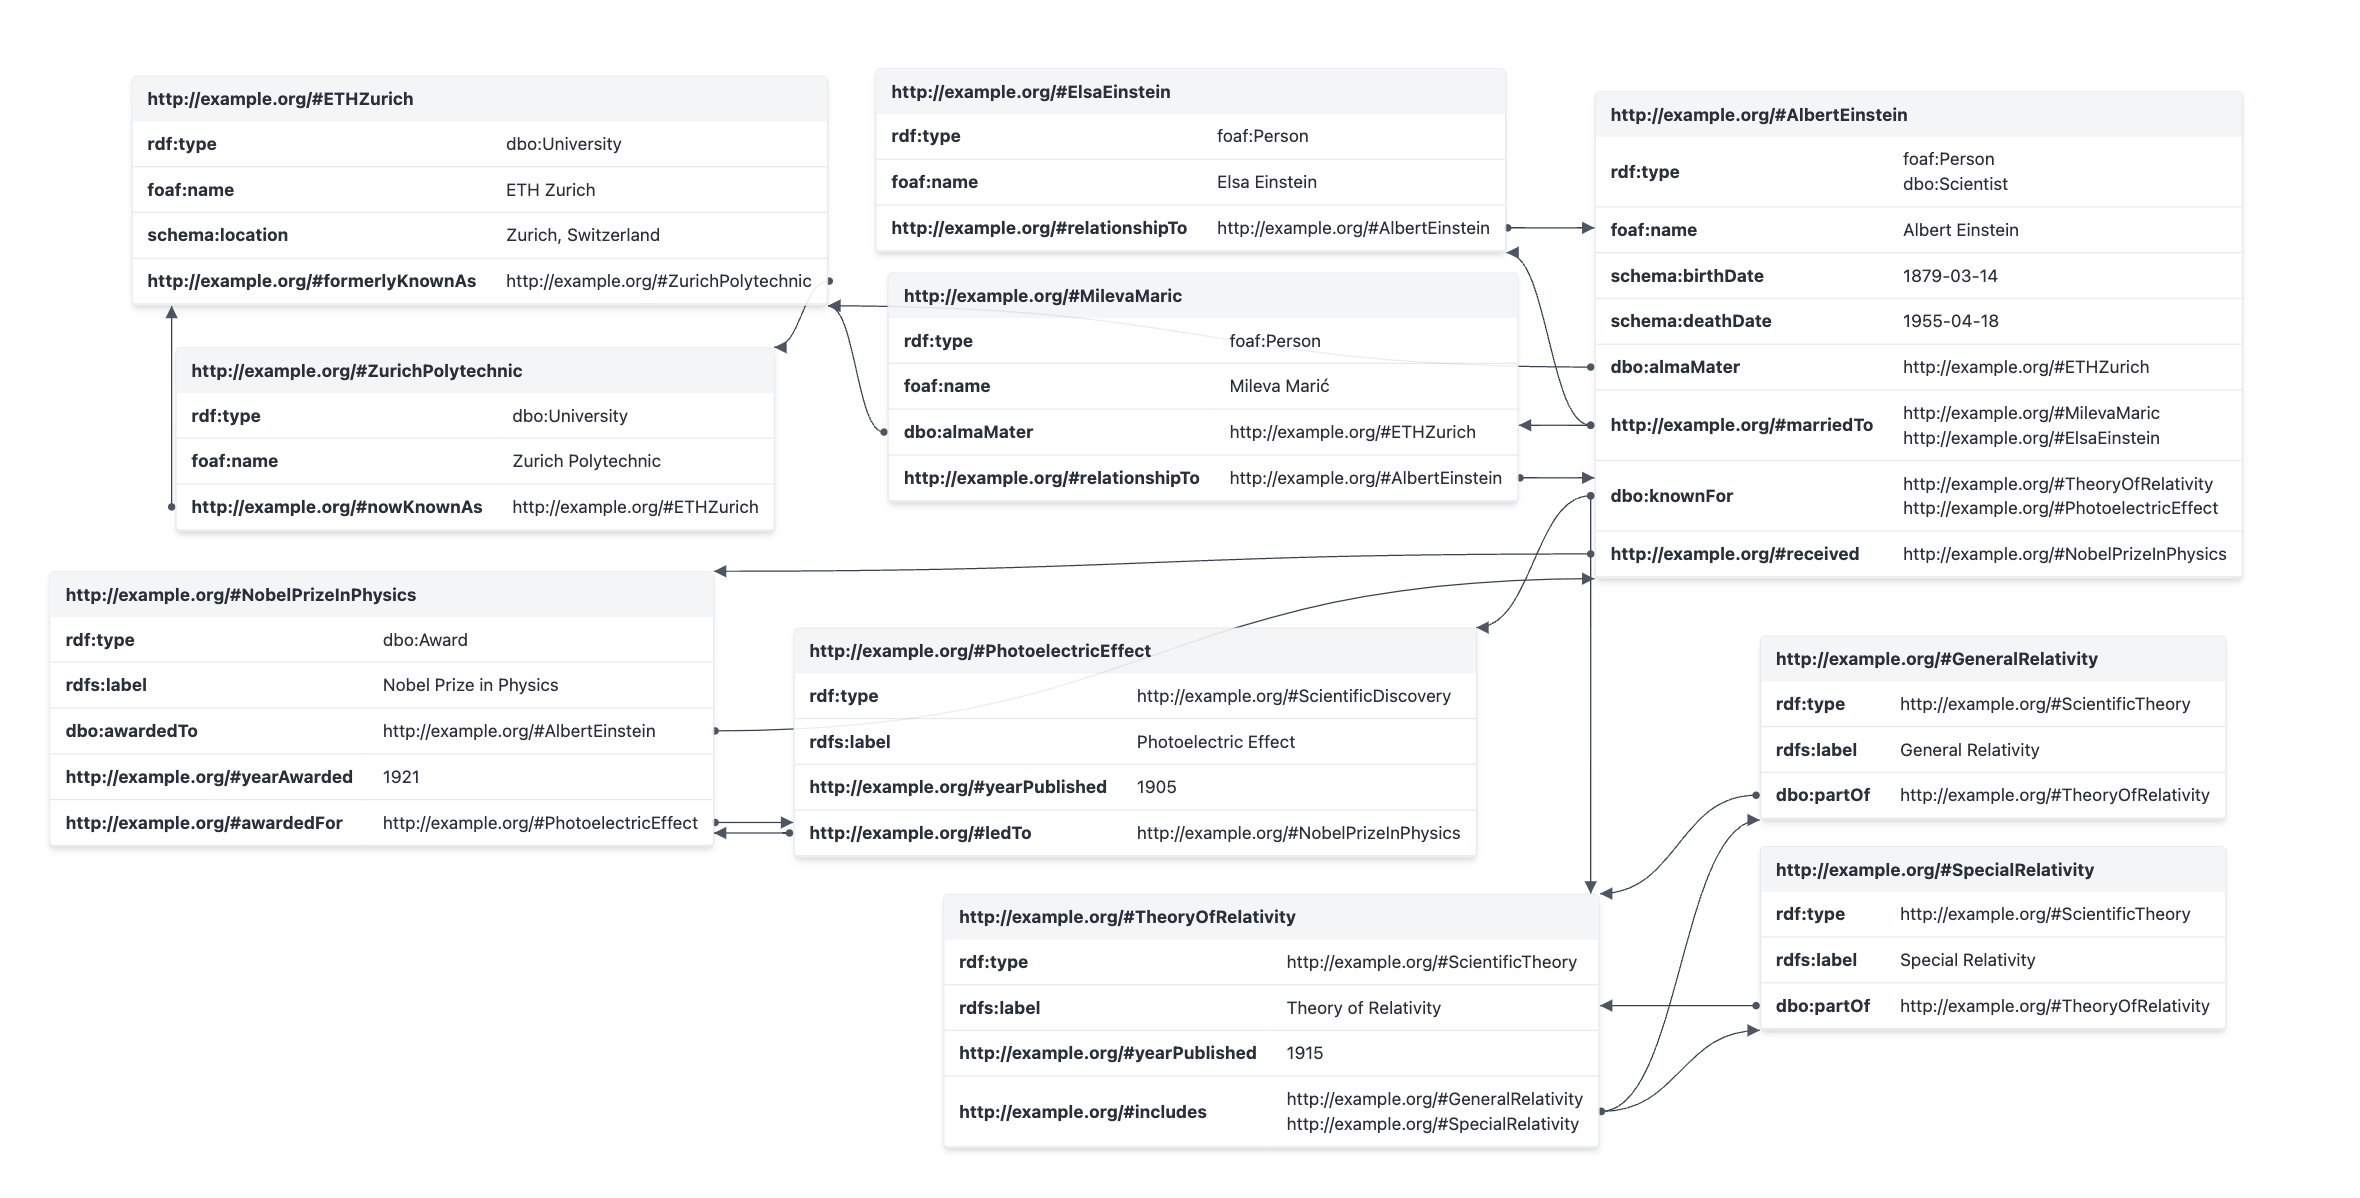
\includegraphics[width=1\textwidth]{5.png}
    \caption{multiple RDF triples, with multiple subjects and objects}
    \label{fig:image5}
\end{figure}

Image 5 show some entities and their relationships. It demonstrates Albert Einstein and relevant data, like the University where he was studying, his participation in research studies, etc.

The code below represents this example in Turtle format:

{\footnotesize
\begin{verbatim}
@prefix rdf: <http://www.w3.org/1999/02/22-rdf-syntax-ns#> .
@prefix rdfs: <http://www.w3.org/2000/01/rdf-schema#> .
@prefix xsd: <http://www.w3.org/2001/XMLSchema#> .
@prefix foaf: <http://xmlns.com/foaf/0.1/> .
@prefix dbo: <http://dbpedia.org/ontology/> .
@prefix schema: <http://schema.org/> .
@prefix : <http://example.org/#> .

:AlbertEinstein a foaf:Person, dbo:Scientist ;
    foaf:name "Albert Einstein" ;
    schema:birthDate "1879-03-14"^^xsd:date ;
    schema:deathDate "1955-04-18"^^xsd:date ;
    dbo:almaMater :ETHZurich ;
    :marriedTo :MilevaMaric, :ElsaEinstein ;
    dbo:knownFor :TheoryOfRelativity, :PhotoelectricEffect ;
    :received :NobelPrizeInPhysics .

:ETHZurich a dbo:University ;
    foaf:name "ETH Zurich" ;
    schema:location "Zurich, Switzerland" ;
    :formerlyKnownAs :ZurichPolytechnic .

:ZurichPolytechnic a dbo:University ;
    foaf:name "Zurich Polytechnic" ;
    :nowKnownAs :ETHZurich .

:MilevaMaric a foaf:Person ;
    foaf:name "Mileva Marić" ;
    :relationshipTo :AlbertEinstein ;
    dbo:almaMater :ETHZurich .

:ElsaEinstein a foaf:Person ;
    foaf:name "Elsa Einstein" ;
    :relationshipTo :AlbertEinstein .

:TheoryOfRelativity a :ScientificTheory ;
    rdfs:label "Theory of Relativity" ;
    :yearPublished "1915"^^xsd:gYear ;
    :includes :GeneralRelativity, :SpecialRelativity .

:GeneralRelativity a :ScientificTheory ;
    rdfs:label "General Relativity" ;
    dbo:partOf :TheoryOfRelativity .

:SpecialRelativity a :ScientificTheory ;
    rdfs:label "Special Relativity" ;
    dbo:partOf :TheoryOfRelativity .

:PhotoelectricEffect a :ScientificDiscovery ;
    rdfs:label "Photoelectric Effect" ;
    :yearPublished "1905"^^xsd:gYear ;
    :ledTo :NobelPrizeInPhysics .

:NobelPrizeInPhysics a dbo:Award ;
    rdfs:label "Nobel Prize in Physics" ;
    dbo:awardedTo :AlbertEinstein ;
    :yearAwarded "1921"^^xsd:gYear ;
    :awardedFor :PhotoelectricEffect .

\end{verbatim}
}

The prefix directives are typically defined at the beginning of the Turtle file. The prefixes are a short version for an IRI. This is done to save space in the file.

\subsubsection{Wikidata}

Wikidata has been chosen as the dataset for this research. It is a free, collaborative, multilingual knowledge base (encyclopedia) that serves as central storage for the structured data of its Wikimedia sister projects, including Wikipedia, Wikivoyage, Wiktionary, and others \citep{vrandecic2014wikidata}. It is published under the CC0 License, meaning that anyone can use the data as they wish.

Wikidata stores data using items and properties. Each item represents a topic (a person, place, or concept) and is assigned a unique identifier. These unique identifiers facilitate the assignment of multiple labels, descriptions, and aliases to an item, which is especially important for multilingual databases. For example, Germany has a UID of Q183. Its names in other languages, such as "Deutschland" or "Германия", also share this UID. On the other hand, when countries change their names, as in the case of "Turkey" becoming "Türkiye", the new name can be aliased while the UID remains the same.

Data in Wikidata is stored in RDF formats, specifically Turtle or N-Triples. Between the subject and object, there is a statement – an entity that contains information about the source from which the information was derived, its rank (indicating trustworthiness), and the date when the statement was added. There is also a direct connection for faster queries.

\begin{figure}[htbp]
    \centering
    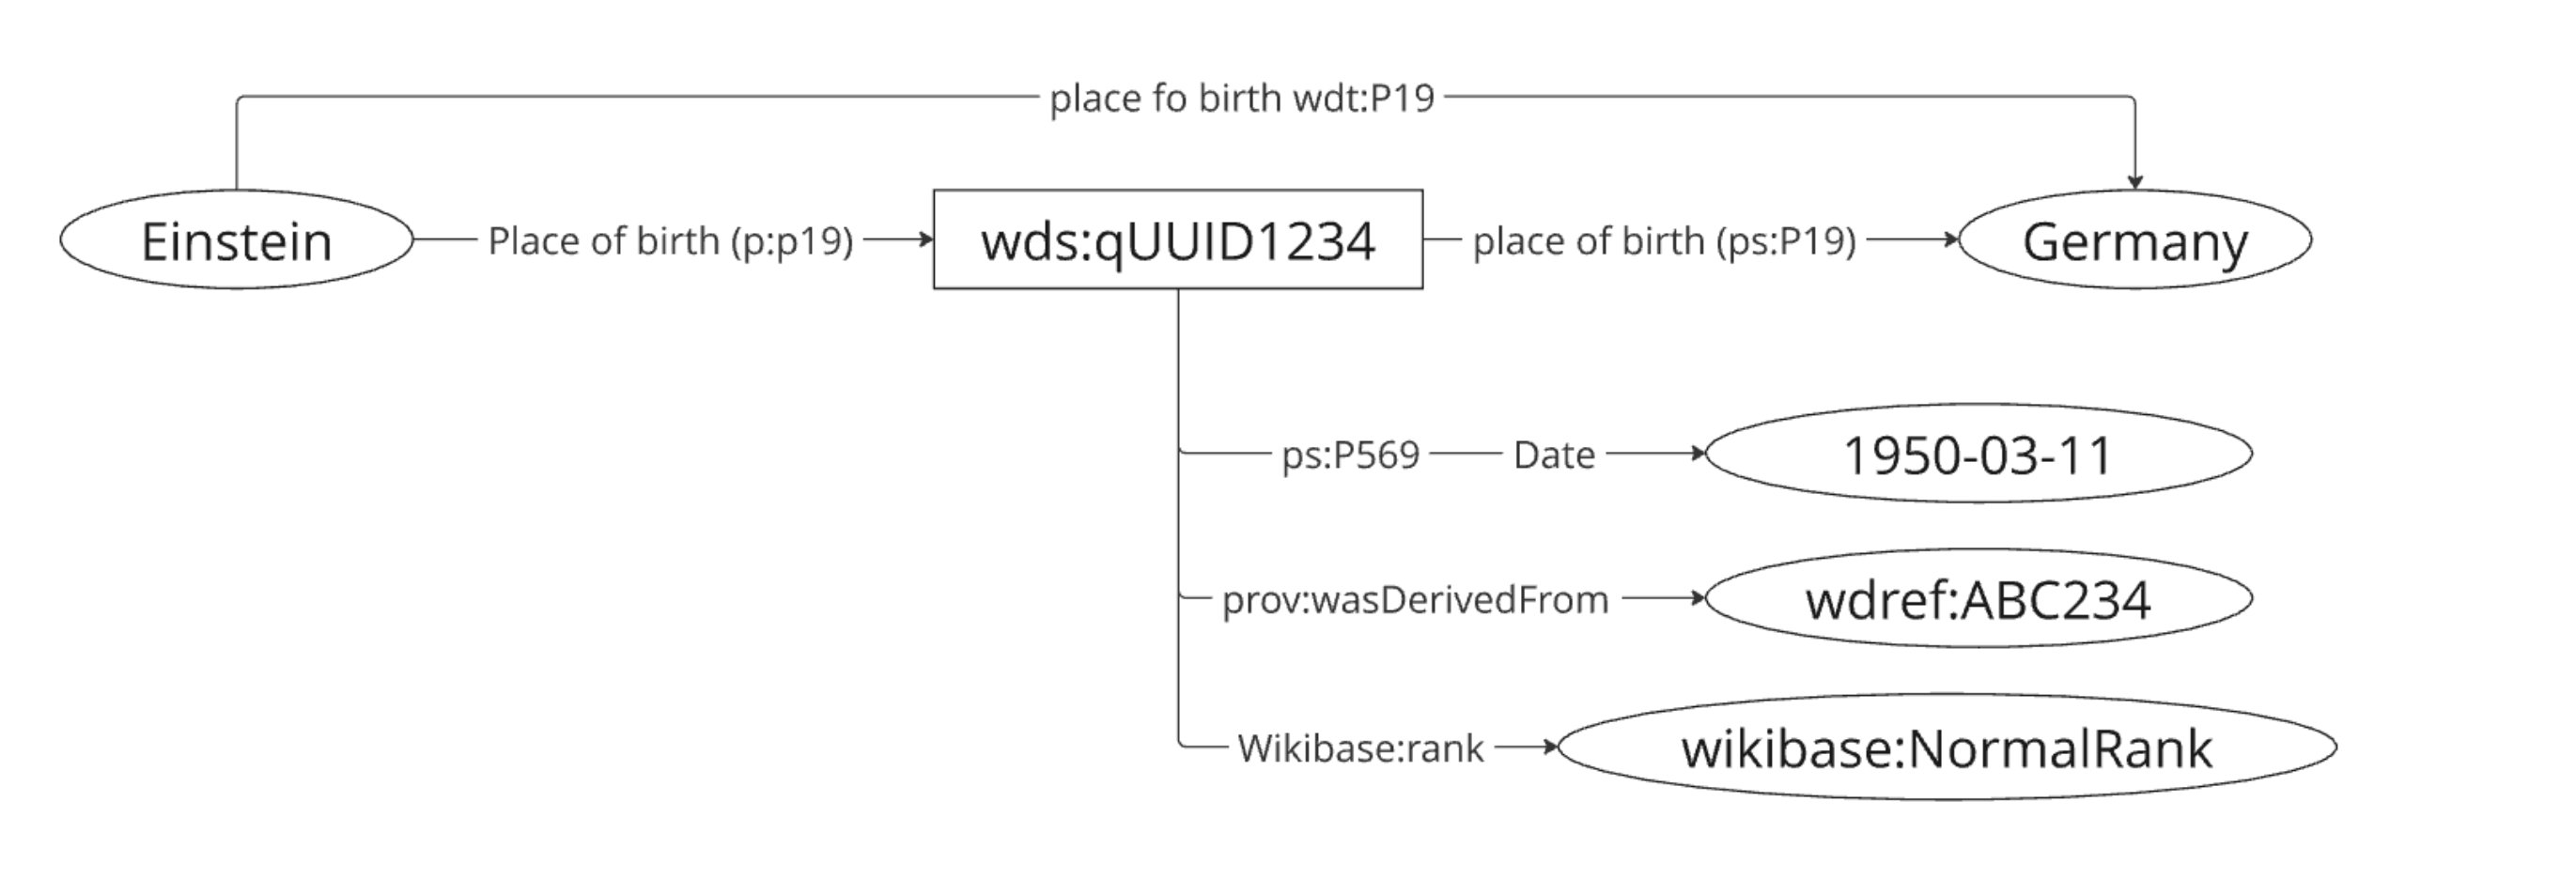
\includegraphics[width=0.8\textwidth]{6.png}
    \caption{Statement structure in Wikidata}
    \label{fig:image6}
\end{figure}

In Wikidata, anyone can edit the existing facts or add new ones. Moderators will then either approve the changes or decline them. To keep track of the data trustworthiness, a ranking system is used: preferred rank – the highest rank that is used to mark the most relevant, up-to-date statement; normal rank – the default rank for a statement that is valid, but not necessarily the most current or preferred; deprecated – the outdated or incorrect data that is kept for historical reasons.

Wikidata contains 140Gb of data in Turtle format \citep{malyshev2018getting}. It is nearly 14.6 billion triples \citep{rdfhdt}.
\subsection{Usage of Statement Qualifiers in Wikidata}

As mentioned earlier, Wikidata contains an extra information between a subject and an object - the statement qualifiers. These qualifiers contain information about the claim's relevancy, date of addition, trustworthiness, and link to a source. Such information is crucial because the facts are provided by users, and the information may be incorrect or uncertain.

\begin{figure}[htbp]
    \centering
    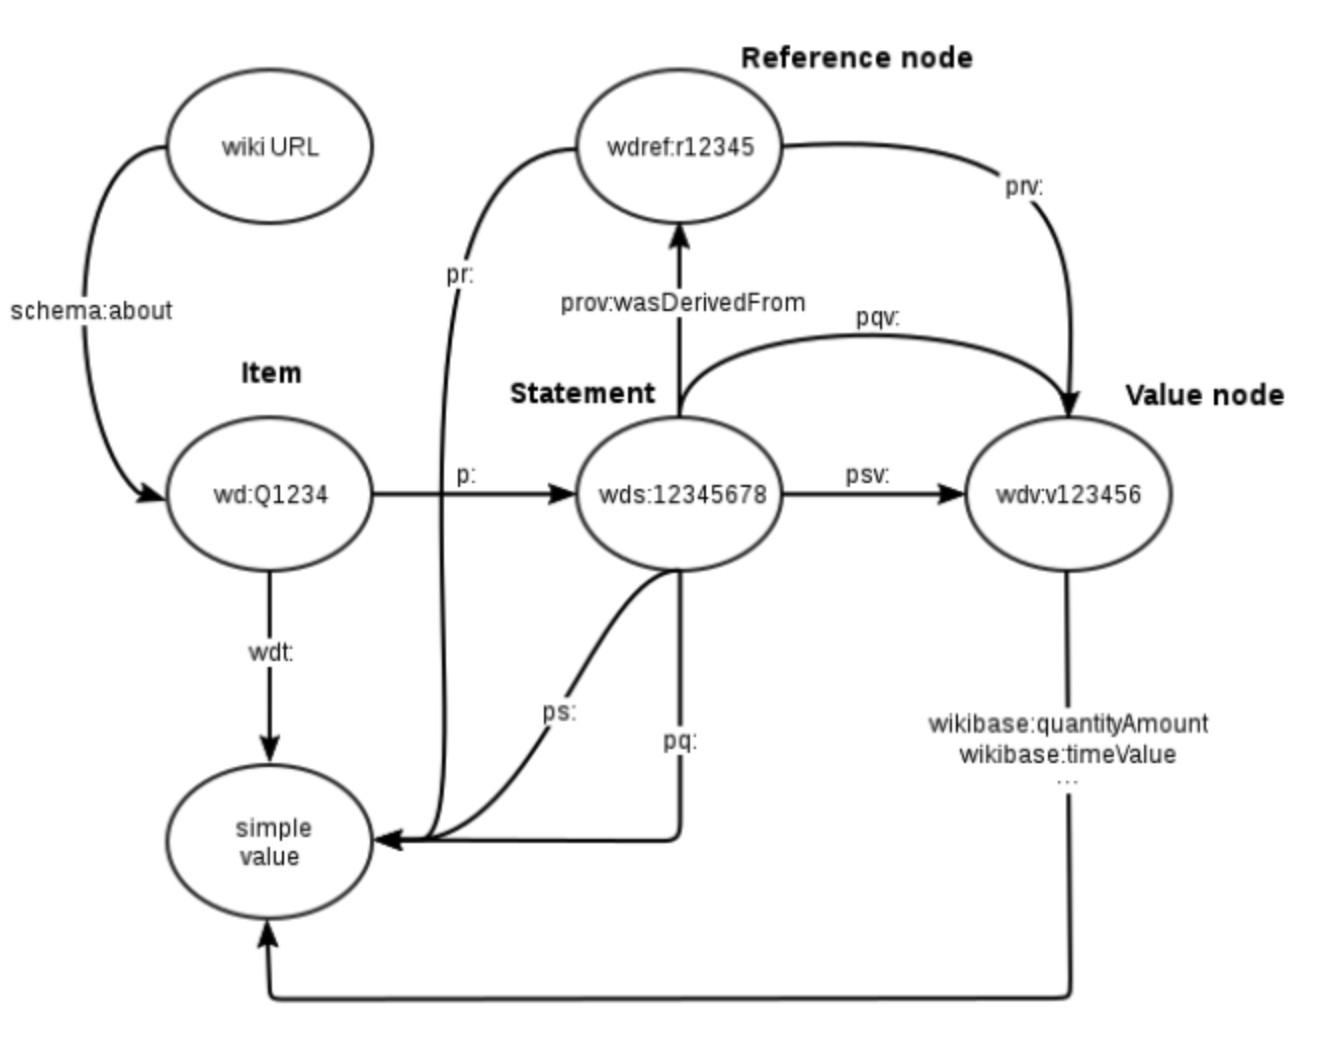
\includegraphics[width=0.5\textwidth]{7.png}
    \caption{Wikidata structure \citep{oxfordsemantic2023wikidata}}
    \label{fig:image7}
\end{figure}

Sometimes there is more than one statement for a given subject-predicate pair. For example, consider the case of citizenships. Einstein, held German, Swiss, and American citizenships. If a user incorrectly added Austrian citizenship and it was mistakenly accepted by moderators, this information would need to be marked as deprecated. The correct citizenship statements would receive either Normal rank (if the fact is certain) or a Preferred rank (if it's considered the most current or relevant).

Qualifiers act as intermediaries between subjects and objects, serving as connectors that provide context and references for the claims. However, to maintain efficiency in data retrieval, Wikidata also maintains direct connections between subjects and objects, allowing for faster queries when detailed information is not required. On the figure 7, there is an example of a statement and its additional nodes. 

\subsubsection{RDF Star (RDF*)}

While RDF is powerful, there are situations where we might want to make statements about other statements. This is where RDF Star, also known as RDF*, comes into play.

RDF* extends the basic RDF model by allowing triples to be treated as resources themselves. This means we can create "triples about triples," which is incredibly useful for adding context or metadata to our statements. This extension addresses a key limitation of standard RDF, where making statements about other statements typically requires complex reification patterns \citep{hartig2017foundations}. 

In RDF*, triples that are the subject or object of other triples are enclosed in double angle brackets (\verb|<<...>>|). This syntax allows for a more intuitive and compact representation of metadata about statements.

Let's consider an example using the Einstein data we've been discussing:

\begin{figure}[htbp]
    \centering
    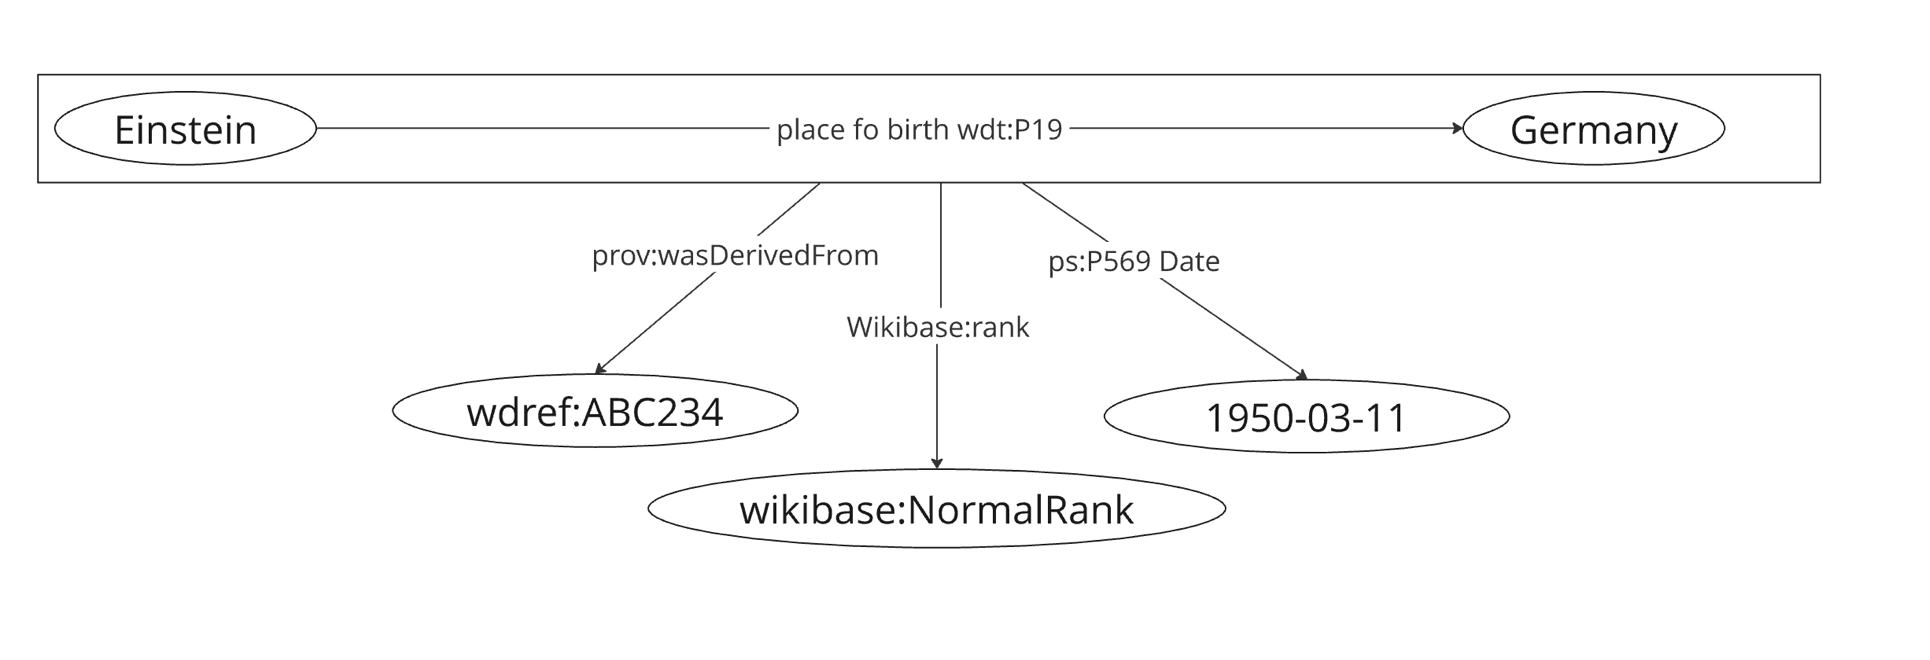
\includegraphics[width=0.8\textwidth]{8.png}
    \caption{RDF* structure in Wikidata}
    \label{fig:image8}
\end{figure}

{\footnotesize
\begin{verbatim}
<<ex:Einstein wdt:P19 ex:Germany>> ps:P569 "1950-03-11"^^xsd:date .
<<ex:Einstein wdt:P19 ex:Germany>> prov:wasDerivedFrom wdref:ABC234 .
<<ex:Einstein wdt:P19 ex:Germany>> wikibase:rank wikibase:NormalRank .
\end{verbatim}
}

The first triple states that the fact Einstein's place of birth (wdt:P19) is Germany was added in 1950. The second triple states that this info was taken from wdref:ABC234, and the third one states that the given triple has a Normal rank.

The huge advantage is that now there are no extra qualified statements that hold the given descriptions of a triple. This RDF* structure directly corresponds to the qualified statements in Wikidata, but in a more compact and intuitive format. It eliminates the need for separate statement nodes, simplifying the data structure while retaining all the necessary information \citep{hartig2017foundations}.

\subsubsection{HDT (Header-Dictionary-Triples)}

\begin{figure}[htbp]
    \centering
    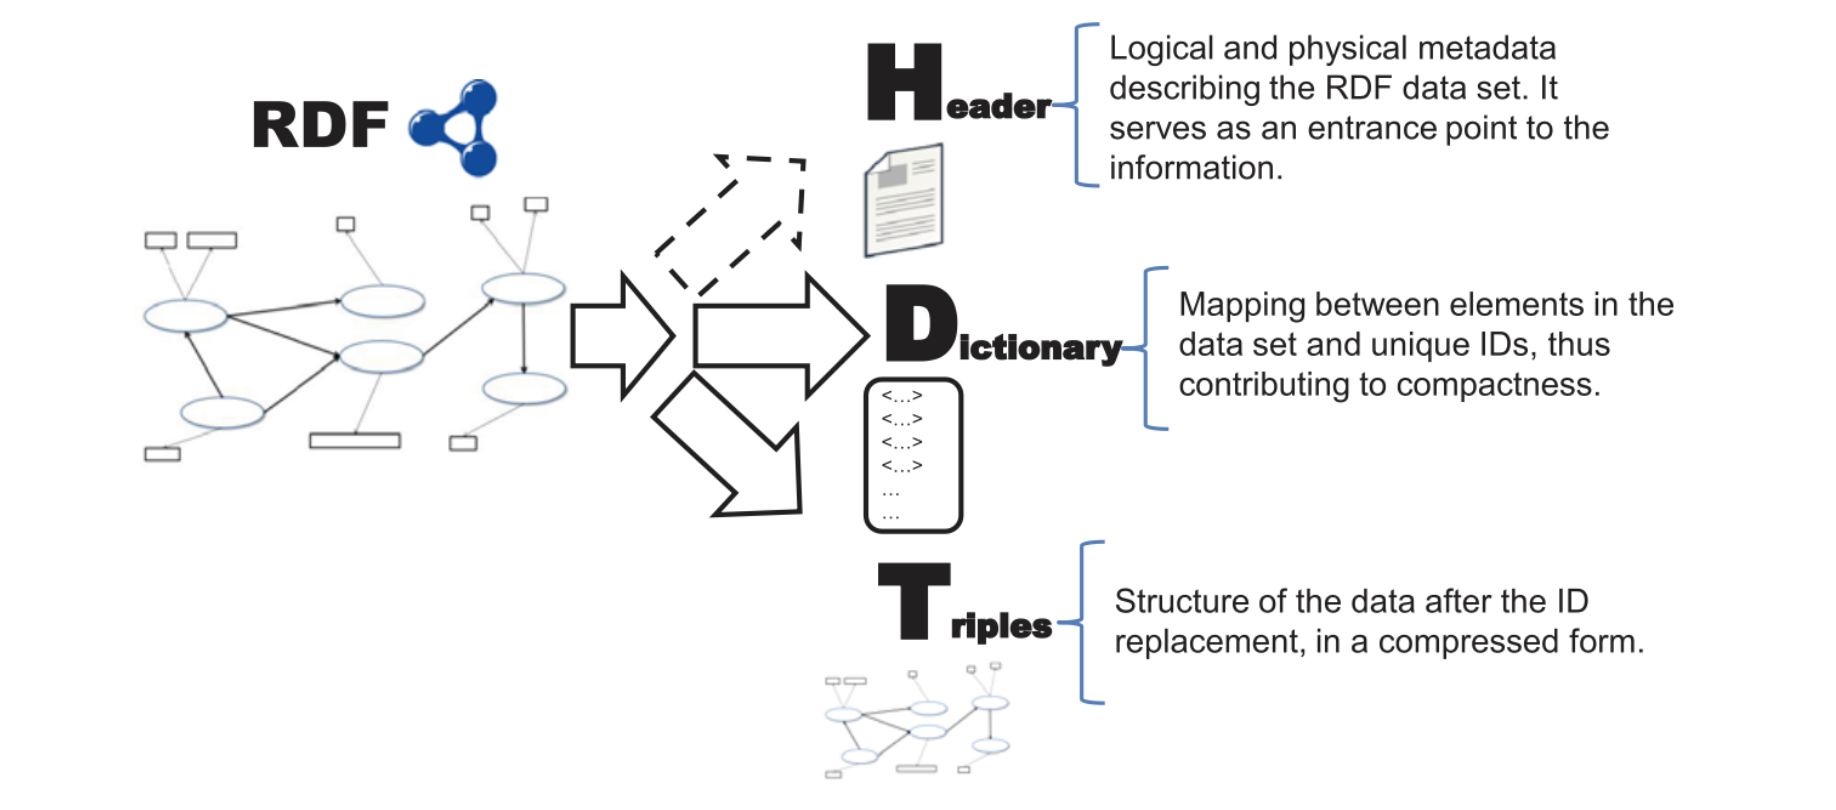
\includegraphics[width=0.8\textwidth]{9.png}
    \caption{HDT structure \citep{fernandez2013binary}}
    \label{fig:image9}
\end{figure}

HDT (Header-Dictionary-Triples) is a binary format designed for the efficient storage and transmission of RDF data \citep{fernandez2013binary}. Think of it as a clever way to compress RDF data without losing the ability to query it efficiently.

% \begin{wrapfigure}{r}{0.5\textwidth}
%     \centering
%     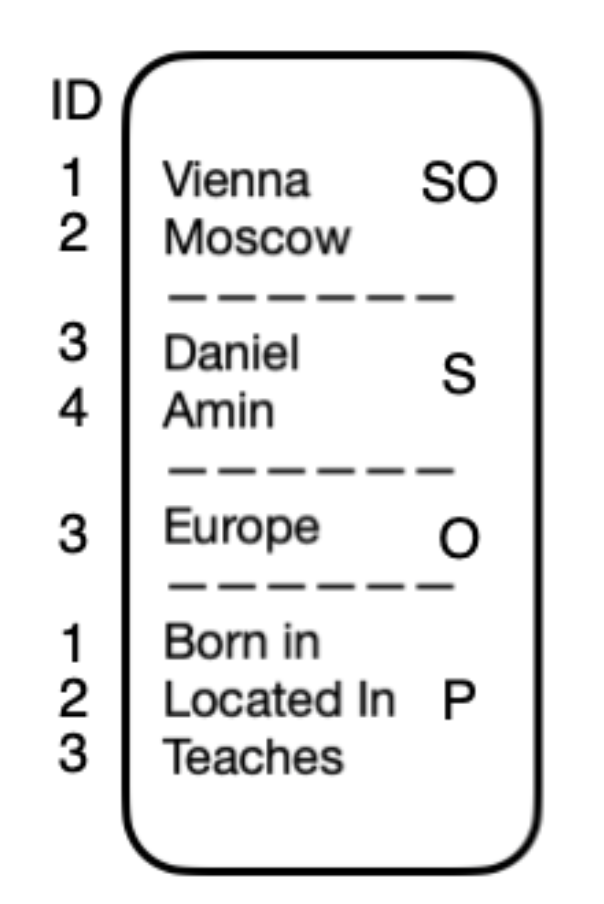
\includegraphics[width=0.4\textwidth]{10.png}
%     \caption{HDT dictionary structure}
%     \label{fig:image10}
% \end{wrapfigure}

\begin{figure}[htbp]
    \centering
    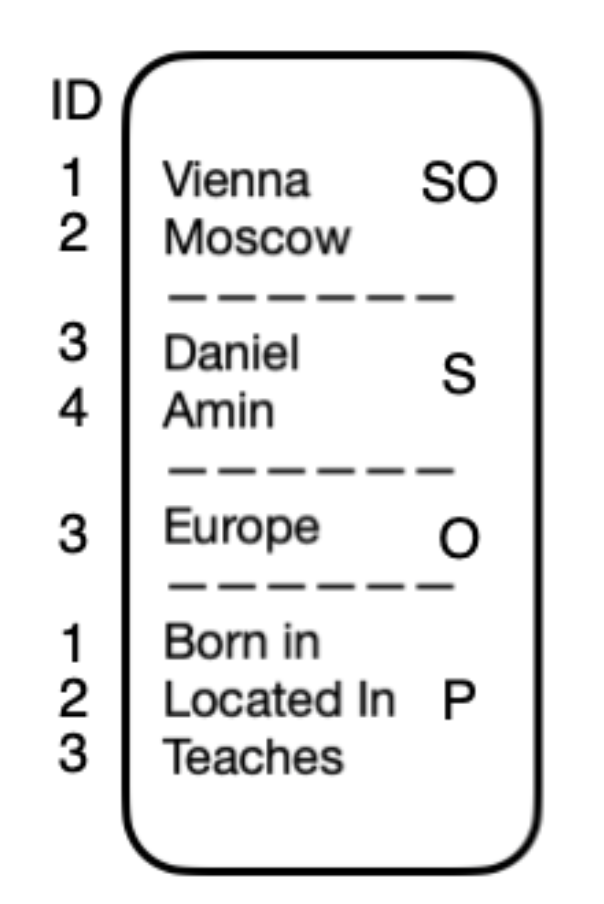
\includegraphics[width=0.4\textwidth]{10.png}
    \caption{HDT dictionary structure}
    \label{fig:image10}
\end{figure}

HDT divides the RDF data into three main components: Header, containing metadata about the dataset \citep{fernandez2018hdtq}. It's like the cover of a book, giving you a quick overview of what's inside; Dictionary – stores all the unique terms (subjects, predicates, and objects) that appear in RDF data. Each term is assigned a unique ID. This approach is useful because it allows HDT to replace long, repetitive strings with short numeric IDs or UUIDs, saving a ton of space. And Triples – stores the actual RDF triples, but instead of using the original terms, it uses the IDs from the dictionary. This makes the triples section very compact.

The magic of HDT lies in how it organizes these components. The dictionary is divided into four sections:


\begin{itemize}
    \item S: for terms that only appear as subjects
    \item O: for terms that only appear as objects
    \item SO: for terms that appear as both subjects and objects
    \item P: for predicates
\end{itemize}

Example on the Figure 10 is a dictionary that is split into four sections. Vienna and Moscow have appeared as subjects (located in Europe) and objects (Daniil Born in Moscow).

This structure, combined with clever encoding techniques, allows HDT to achieve impressive compression rates while still allowing for efficient querying.

For example, if we have many triples about Albert Einstein, the string \verb|"Albert_Einstein"| is stored only once in the dictionary and assigned an ID, let's say 937. Then in the triples section, we'd just use 937 wherever "Albert\_Einstein" appears as a subject or object. This saves a lot of space, especially for large datasets with many repeated terms.

But HDT isn't just about saving space. Its structure also allows for efficient query resolution \citep{fernandez2018hdtq}. When you want to find all triples about Albert Einstein, HDT can quickly locate the ID for "Albert\_Einstein" in the dictionary and then find all triples with that ID in the subject position.

\subsection{SPARQL, Querying RDF Data}

SPARQL is an RDF Query language, that is similar to SQL for relational data. It allows users to write queries to the data, that follows RDF specification \citep{harris2013sparql}. The structure of SPARQL query resembles the query format of RDF. It typically consists of a set of triple patterns called a basic graph pattern. These patterns are similar to RDF triples, but with the option of placing a variable in the subject, predicate, or object position. This flexibility allows for complex queries that can extract specific information from large RDF datasets. For example, a simple SPARQL query to find all of Einstein's discoveries might look like:

{\footnotesize
\begin{verbatim}
SELECT ?discovery
WHERE {
    ex:Einstein dbo:knownFor ?discovery .
}
\end{verbatim}
}

SPARQL is suitable for more complex queries. It can make filtering, ordering or aggregation of results. It can also be used to modify or construct the RDF data in a chosen format \citep{perez2009semantics}.

% SPARQL is not limited to retrieving data; it can also modify existing RDF data and construct new RDF graphs. The language includes four main types of queries: SELECT for retrieving raw values from a SPARQL endpoint, CONSTRUCT for creating RDF graphs, ASK for simple True/False queries, and DESCRIBE for retrieving RDF graphs that describe resources. The CONSTRUCT query, in particular, is powerful for transforming data from one vocabulary to another or for generating new triples based on existing data patterns \citep{angles2008expressive}.

% Recent research has explored ways how SPARQL could be more efficient and suitable for other types of data \citep{frey2019rewriting}. One of them is rewriting SPARQL queries based on RDF schema to RDF* schema \citep{hartig2017foundations}.

% That means, that SPARQL queries are not ideal and can be more efficient with specific approach.

\section{Problems of RDF adressing Wikidata data structure}

Scale and complexity of linked data continue to grow, particularly in large-scale knowledge bases such as Wikidata, therefore, several critical challenges emerge in the management and querying of RDF data \citep{fernandez2018hdtq}. This research addresses three primary issues that significantly impact the efficiency and expressiveness of current RDF data models.

\subsection{Challenges of RDF*}

The main challenge in serialisation RDF* into existing RDF data models lies in the increased complexity it introduces, particularly when dealing with large-scale knowledge bases like Wikidata. While RDF* extends the standard RDF model to allow triples to be treated as subjects or objects in other triples, this capability, paradoxically, can lead to more convoluted data structures.

In the context of Wikidata, the use of RDF* to represent qualified statements results in a proliferation of nested triples. Each piece of metadata about a statement - such as its date, rank, or reference - requires an additional RDF* triple. This leads to a significant increase in the number of triples needed to represent even simple facts, as the same base triple is repeated for each metadata element. The redundancy not only increases storage requirements but also complicates query processing.

Furthermore, the current implementations of RDF* often treat it as an adjunct feature rather than a core component of the data model. This approach limits the potential benefits of RDF* in representing complex, nested information structures efficiently. The lack of native support for RDF* in many RDF stores and query systems results in inefficient encoding of metadata about statements, missing opportunities for more compact and semantically rich data representations.

The challenge, therefore, is to develop a method that can leverage the expressive power of RDF* while avoiding the pitfalls of increased complexity and redundancy. The solution needs to provide a more streamlined approach to representing metadata and qualified statements, without sacrificing the rich contextual information that makes RDF* valuable. This is particularly crucial for resources, like Wikidata, where the volume of metadata can quickly overwhelm the base data if not managed efficiently.

\subsection{Challenges of RDF in Wikidata”}

This challenge concerns the use of qualified statements in Wikidata and in other similar structures. These statements provide valuable contextual information, including data provenance and reliability metrics, however they introduce inefficiencies in both storage and query processing.

Qualified statements in Wikidata function as intermediary nodes between subjects and objects, necessitating additional steps in data retrieval processes. “For example, as illustrated in Figure 6, a Statement in Wikidata employs an intermediary node to connect the subject <<Einstein>> with the object <<Germany>> while incorporating additional metadata such as rank and references. This intermediary node requires queries to navigate through an extra layer, increasing both storage demands and query complexity. The redundancy inherent in storing these intermediary nodes for each subject-object relationship results in a significant expansion of the data volume, which becomes particularly problematic at the scale of Wikidata.

Moreover, the presence of these qualified statements complicates query execution. Each data retrieval operation must navigate through these additional nodes, potentially traversing multiple levels of metadata. This increased path length in query resolution can lead to substantial performance degradation, especially in complex queries involving multiple relationships or highly connected entities.

\subsection{Temporal and Repeated Relationship Representation – "Marriage problem"}

The third challenge, which we term the "marriage problem," addresses the limitations of current RDF models in representing temporal data and repeated relationships between entities. This issue is exemplified by scenarios such as multiple marriages between the same individuals over time.

RDF* triples lack inherent mechanisms for distinguishing between multiple instances of the same relationship type occurring at different times. For instance, in representing multiple marriages between two individuals, the RDF statement "Person A married Person B" may appear multiple times without clear temporal differentiation. This limitation extends to various domains where relationships between entities evolve over time or occur repeatedly.

The inability to efficiently encode and query such temporal and repeated relationship data within RDF* framework poses significant challenges. It complicates data interpretation, hinders accurate temporal analysis, and can lead to ambiguities in knowledge representation. Furthermore, this limitation impacts the effectiveness of querying historical data or tracking the evolution of relationships over time.

These three challenges – the inefficiency of qualified statements, suboptimal RDF* integration, and inadequate representation of temporal and repeated relationships – form the core focus of this research. Addressing these issues is crucial for enhancing the efficiency, expressiveness, and analytical capabilities of large-scale RDF data management systems, particularly in the context of evolving knowledge bases like Wikidata.

The subsequent sections of this thesis will explore our proposed approach to mitigate these challenges, proposing innovations in RDF data modelling, storage, and querying techniques. These proposed solutions aim to improve the performance and expressiveness of RDF-based knowledge representation systems, paving the way for more efficient and capable linked data infrastructures.

To illustrate this challenge, let's consider a fictional example of Einstein's marriages represented in RDF and RDF*. In standard RDF, we might have:

\begin{figure}[htbp]
    \centering
    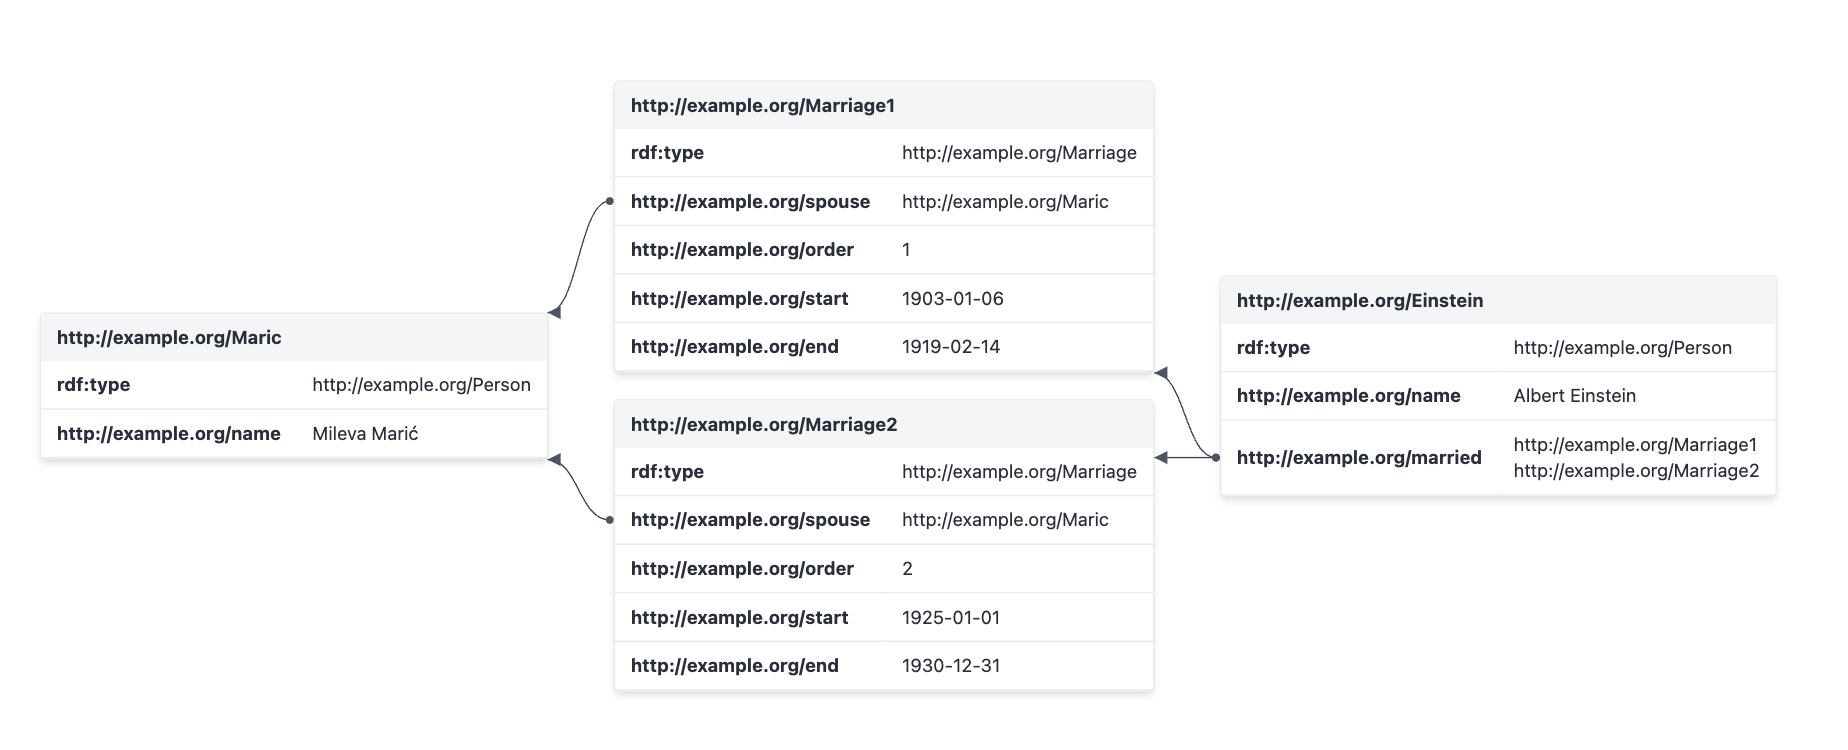
\includegraphics[width=0.8\textwidth]{11.png}
    \caption{Property Graph Representing Marriage Problem}
    \label{fig:image11}
\end{figure}

{\footnotesize
\begin{verbatim}
<Einstein> <married> <Mileva Marić> .
<Einstein> <married> <Mileva Marić> .
\end{verbatim}
}

This representation fails to capture the temporal aspect and doesn't distinguish between the two marriages. It's unclear whether this represents two separate marriages or a data error. RDF* attempts to address this by allowing metadata about triples:

{\footnotesize
\begin{verbatim}
<<Einstein married Mileva Marić>> <startDate> "1903"^^xsd:date .
<<Einstein married Mileva Marić>> <endDate> "1919"^^xsd:date .
<<Einstein married Mileva Marić>> <startDate> "1925"^^xsd:date .
<<Einstein married Mileva Marić>> <endDate> "1930"^^xsd:date .
\end{verbatim}
}

While this provides more information, it introduces new problems. The same triple ("Einstein married Mileva Marić") is used for both marriages, leading to potential confusion. It's not immediately clear which start and end dates correspond to which marriage. This approach also introduces redundancy, as the base triple is repeated for each piece of metadata.

To maintain order and clarity, additional statements or complex querying would be necessary, further complicating the data structure and retrieval process. We don't want to create additional statements for this purpose, as it would make the graphs more complex and harder to manage.

The inability to efficiently encode and query such temporal and repeated relationship data within the RDF framework poses significant challenges. It complicates data interpretation, hinders accurate temporal analysis, and can lead to ambiguities in knowledge representation. Furthermore, this limitation impacts the effectiveness of querying historical data or tracking the evolution of relationships over time.

These challenges – the inefficiency of qualified statements, suboptimal RDF* integration, and inadequate representation of temporal and repeated relationships – form the core focus of this research. Addressing these issues is crucial for enhancing the efficiency, expressiveness, and analytical capabilities of large-scale RDF data management systems, particularly in the context of evolving knowledge bases like Wikidata.

The subsequent sections of this thesis will explore novel approaches to mitigate these challenges, proposing innovations in RDF data modelling, storage, and querying techniques. 

% These proposed solutions aim to significantly improve the performance and expressiveness of RDF-based knowledge representation systems, paving the way for more efficient and capable linked data infrastructures.


\section{Proposed Approaches}
In the thesis we try to solve the problems, answering two research questions discussed berfore. First, we started with answering of the first question: Whether it is possible to represent RDF* in a form of HDT, we tried to address problems, described in the previous part. While creating the converter to HDT from RDF* (named by us as HDT*), we came up with different struggled, concerning the structure, and specifically the marriage problem. In the next subsections we will take a closer look at the issues of HDT*.

The uncertainties and issues of HDT* lead us to inventing new form of HDT, that solves all of the issues, remaining in the HDT. The revised approach will be explained afther the following subsection.

\subsection{Initial Approach: HDT Star}

Our initial approach to addressing the challenges of managing large-scale RDF data, particularly from Wikidata, involved developing a new serialisation format we call HDT Star (HDT*). This section details our methodology, the rationale behind our decisions, and the challenges we encountered during this process.

The primary motivation for developing HDT* was to combine the compression and query efficiency of the HDT format with the expressive power of RDF*. Standard HDT lacks native support for the nested triple structures that RDF* introduces. Our goal was to create a format that could efficiently handle the complex metadata structures present in datasets like Wikidata, without sacrificing the performance benefits that make HDT attractive.

\subsubsection{Methodology}

We aimed to extend HDT to support RDF* capabilities, maintain or improve upon HDT's compression ratios, ensure efficient query performance for RDF* structures, and preserve backward compatibility with standard HDT as much as possible. To achieve these goals, we developed a two-step approach. The first step involved converting the standard Wikidata Turtle RDF file into an RDF* format. This process allowed us to represent metadata about statements directly within the RDF structure, addressing some of the limitations of standard RDF in representing complex relationships and metadata. The second step involved two parallel processes: converting the original Wikidata Turtle RDF file to standard HDT format and converting our newly created Wikidata Turtle RDF* file to the new HDT* format.

% \begin{wrapfigure}{r}{0.6\textwidth}
%     \centering
%     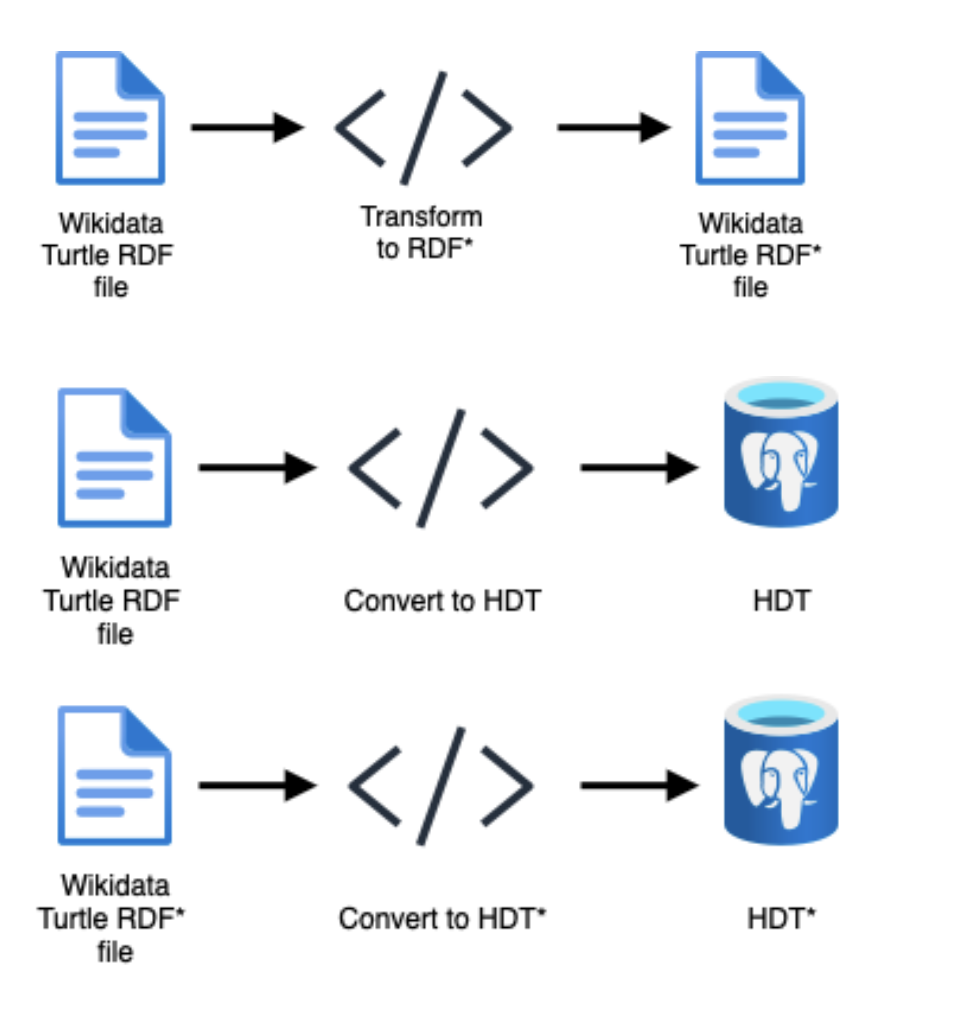
\includegraphics[width=0.4\textwidth]{12.png}
%     \caption{RDF* to HDT* and comparison with RDF and HDT}
%     \label{fig:image12}
% \end{wrapfigure}

\begin{figure}[htbp]
    \centering
    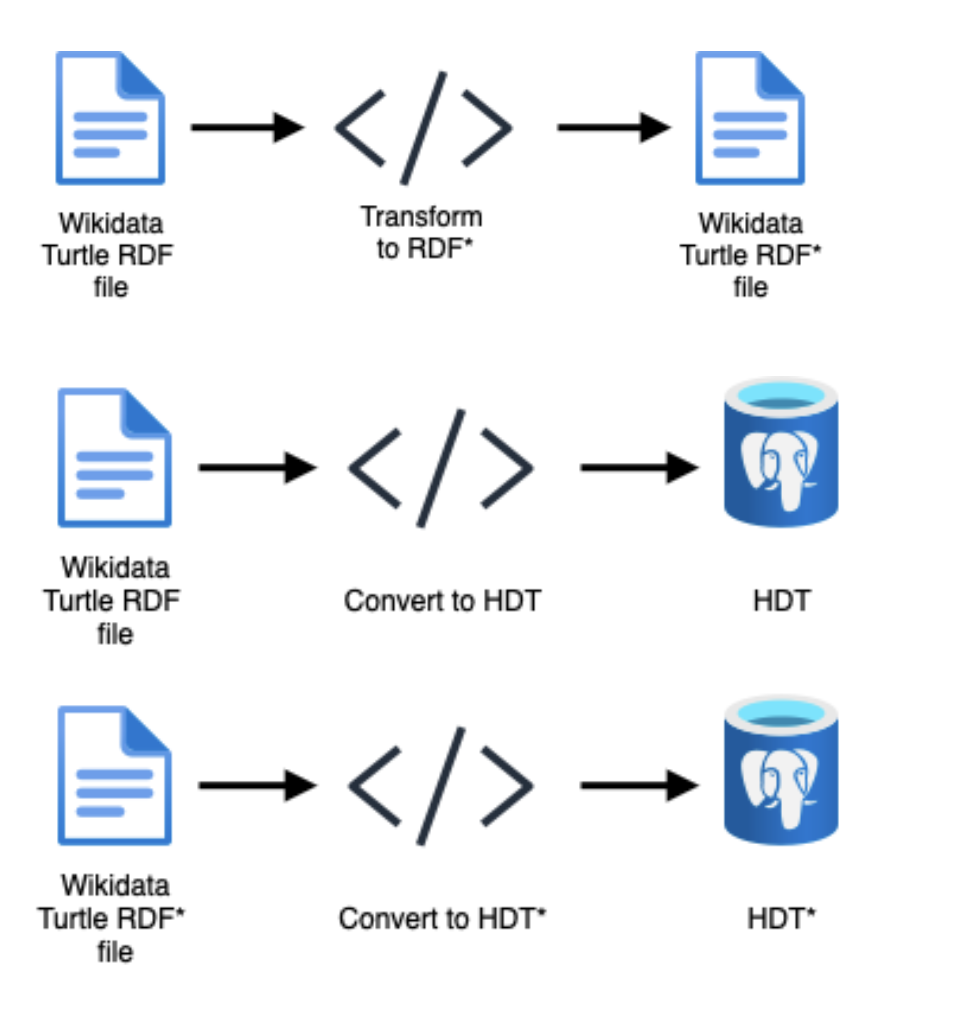
\includegraphics[width=0.5\textwidth]{12.png}
    \caption{RDF* to HDT* and comparison with RDF and HDT}
    \label{fig:image12}
\end{figure}

To transform the standard RDF data into RDF*, we developed a Python script that processes the Wikidata Turtle file. The script reads the input file line by line, identifying triples and their associated metadata. For each triple, it checks if there are associated metadata triples (e.g., qualifiers, references). When metadata is found, the script constructs an RDF* triple by nesting the original triple within angle brackets and adding the metadata as properties of this nested triple. The transformed triples are then written to a new Turtle file in RDF* format.

This transformation process presented several challenges. The entire Wikidata dump is approximately 140Gb \citep{wikidata_dumps}, which requires significant computational resources and time to process. Wikidata's data model includes various types of metadata (qualifiers, ranks, references) that needed to be correctly represented in RDF*. Ensuring that all related metadata was correctly associated with its corresponding triple required careful tracking of statement identifiers.

With both standard RDF and RDF* versions of the Wikidata data, we proceeded to convert these into HDT and HDT* formats respectively. For the standard HDT conversion, we used existing HDT tools: hdt-it \citep{hdtit} and rdf2hdt \citep{rdf2hdt}. This process involves creating a dictionary by assigning unique identifiers to all subjects, predicates, and objects in the dataset, encoding triples using the assigned identifiers, and generating bitmap structures for efficient querying.

Developing the HDT* format required modifications to the standard HDT conversion process. We extended Subject dictionary by embedding RDF* triples, allowing nested triples to be indexed alongside standard triples without altering the overall HDT structure.

\subsubsection{Design Decisions}

In designing HDT*, we faced several key decisions. For extending the HDT dictionary to support RDF*, we considered two main approaches: adding a new column specifically for storing RDF* triples or incorporating RDF* triples into the existing S, O, or SO columns. After careful consideration, we chose to incorporate RDF* triples into the S column. This decision was based on minimizing changes to the existing HDT structure, leveraging existing efficient lookup mechanisms for the S column, and reducing the potential for dictionary bloat.

The Triples section required minimal changes. Since we represent RDF* triples with integer IDs from the Dictionary (just like regular terms), they fit well into the existing BitmapTriples structure. This decision helped maintain compatibility with standard HDT and simplified query processing. To support querying of RDF* data, we had to extend the query mechanisms. This involved modifying dictionary lookup procedures to handle nested triples, adjusting query parsing to understand RDF* patterns, and developing new strategies to optimize complex queries involving nested structures.

\subsubsection{Challenges and Limitations}

During the development of HDT*, we faced several significant challenges. Including entire RDF* triples in the dictionary had the potential to significantly increase its size. We had to carefully balance this against the benefits of RDF* expressiveness. Queries involving nested triples are inherently more complex, and we had to figure out how to execute these queries efficiently without sacrificing the performance gains that make HDT attractive. Maintaining backward compatibility with regular HDT while adding new features was a delicate balance.

To implement and test our HDT* approach, we used Python for developing the RDF to RDF* conversion script and initial HDT* prototype. We also used PostgreSQL to store HDT and HDT* structures for initial testing and comparison.

However, as we progressed with our implementation and conducted initial tests on a small 1Mb subset of the Wikidata dataset, we encountered a significant obstacle. The "marriage problem" - the difficulty in representing multiple instances of the same relationship type efficiently - proved to be a major challenge that RDF* and, by extension, our HDT* approach, struggled to solve effectively. This issue, along with other related problems in representing complex temporal and repeated relationships, forced us to reevaluate our approach.

% The other significant issue was to store blank nodes in the new HDT format. Some of the solutions may have been creating a special subject that would relate to the blank node. it can be either Skolemization – where each blank node is assigned a globally unique IRI, or creating internal indendifiers for the blank nodes within the HDT* dictionary.

\subsubsection{Reevaluation of Approach}

Our approach was to represent triples as subjects to give description to it. For that, some triples had to be added into the Dictionary: either a new section or to the subject section. 

We realized that while RDF* offered improved expressiveness over standard RDF, it still fell short in addressing some of the fundamental challenges posed by datasets like Wikidata. The nested structure of RDF*, while useful in many scenarios, did not provide an elegant solution to the "marriage problem" without introducing additional complexities or redundancies.

This realization led us to question whether RDF* was indeed the best approach for our purposes. It became clear that to truly solve problems like the "marriage problem", we would need to think beyond the constraints of RDF* and consider alternative approaches to representing and storing RDF data.

As a result, we made the difficult decision to halt our development of HDT*. Instead of continuing down a path that we now recognized had inherent limitations, we decided to step back and reconsider our approach from a more fundamental level. We began to explore whether there might be other solutions that could address the challenges we faced without relying on RDF*.

% This pivot in our research direction was a crucial moment. It highlighted the importance of remaining flexible and open to new ideas, even when significant work has already been invested in a particular approach. By acknowledging the limitations of RDF* and HDT* in solving the specific problems we encountered, we opened ourselves up to exploring more innovative and potentially more effective solutions.

In the next section, we will discuss the revised methodology that emerged from this realization. This new approach moves away from the nested structure of RDF* and instead focuses on using indexed predicate chains. By learning from the challenges we encountered with HDT*, we were able to design a more tailored solution that better fits the specific needs of large-scale, metadata-rich RDF datasets like Wikidata, particularly in addressing issues like the "marriage problem" that proved so challenging in our initial approach.

% First, the research topic was to implement RDF* in the HDT format. That would have helped to store data in structured form. All triple elements: Subjects, Predicates, Objects would have been saved in the Dictionary table and their encoded names would have been written in the Triples section. The size of the HDT file would have been much smaller, that Turtle or NT format. However, in standard HDT, there is not possibility to use RDF* – the description of a triple.

% To convert HDT to HDT*, there has to be a possibility to give a description to a triple. There are multiple ways to implement RDF*. For example, researchers in Vienna University of Economics and Business et. Al, created HDTQ format. The difference between HDT and HDTQ is that HDTQ has Quads instead of triples \citep{fernandez2018hdtq}. Here 2 variants of storing appear: either to add extra column to add an optional description for each triple. Or, to add an additional section Q, where the triples together with the description will be written.

\subsection{Revised Approach: Indexed Property Chains}

% While working on the conversion of Wikidata to HDT format, it became clear that the existing methods, including RDF*, presented significant challenges. The primary issue lay in handling Wikidata's complex statement structure, and the problem, known as the "marriage problem" - the difficulty in representing multiple instances of the same relationship type efficiently. Therefore we decided to find a novel approach to RDF data representation.

The proposed method introduces a new way of storing RDF data using chains of predicates and indexed values. This approach aims to eliminate the need for intermediary statement nodes while maintaining the rich context and provenance information crucial for knowledge bases like Wikidata. Moreover, such approach creates a hierarchy with enumerated nodes, that solves the marriage problem.

In the new format, predicates that form a path between a subject and an object are chained together. For example, instead of using separate triples connected by a statement node, we use a single triple with a chain of predicates:

{\footnotesize
\begin{verbatim}
wd:Q42 <p:P19|ps:P19>[1,1] wd:Q183
Einstein <p:PlaceOfbirth>[1] Germany
\end{verbatim}
}

Here, wd:Q42 represents Einstein, p:P19|ps:P19 is a chain of predicates indicating "place of birth", and wd:Q183 represents Germany. The number in brackets which follows the property chains is an index, which we'll explain further.

\begin{figure}[htbp]
    \centering
    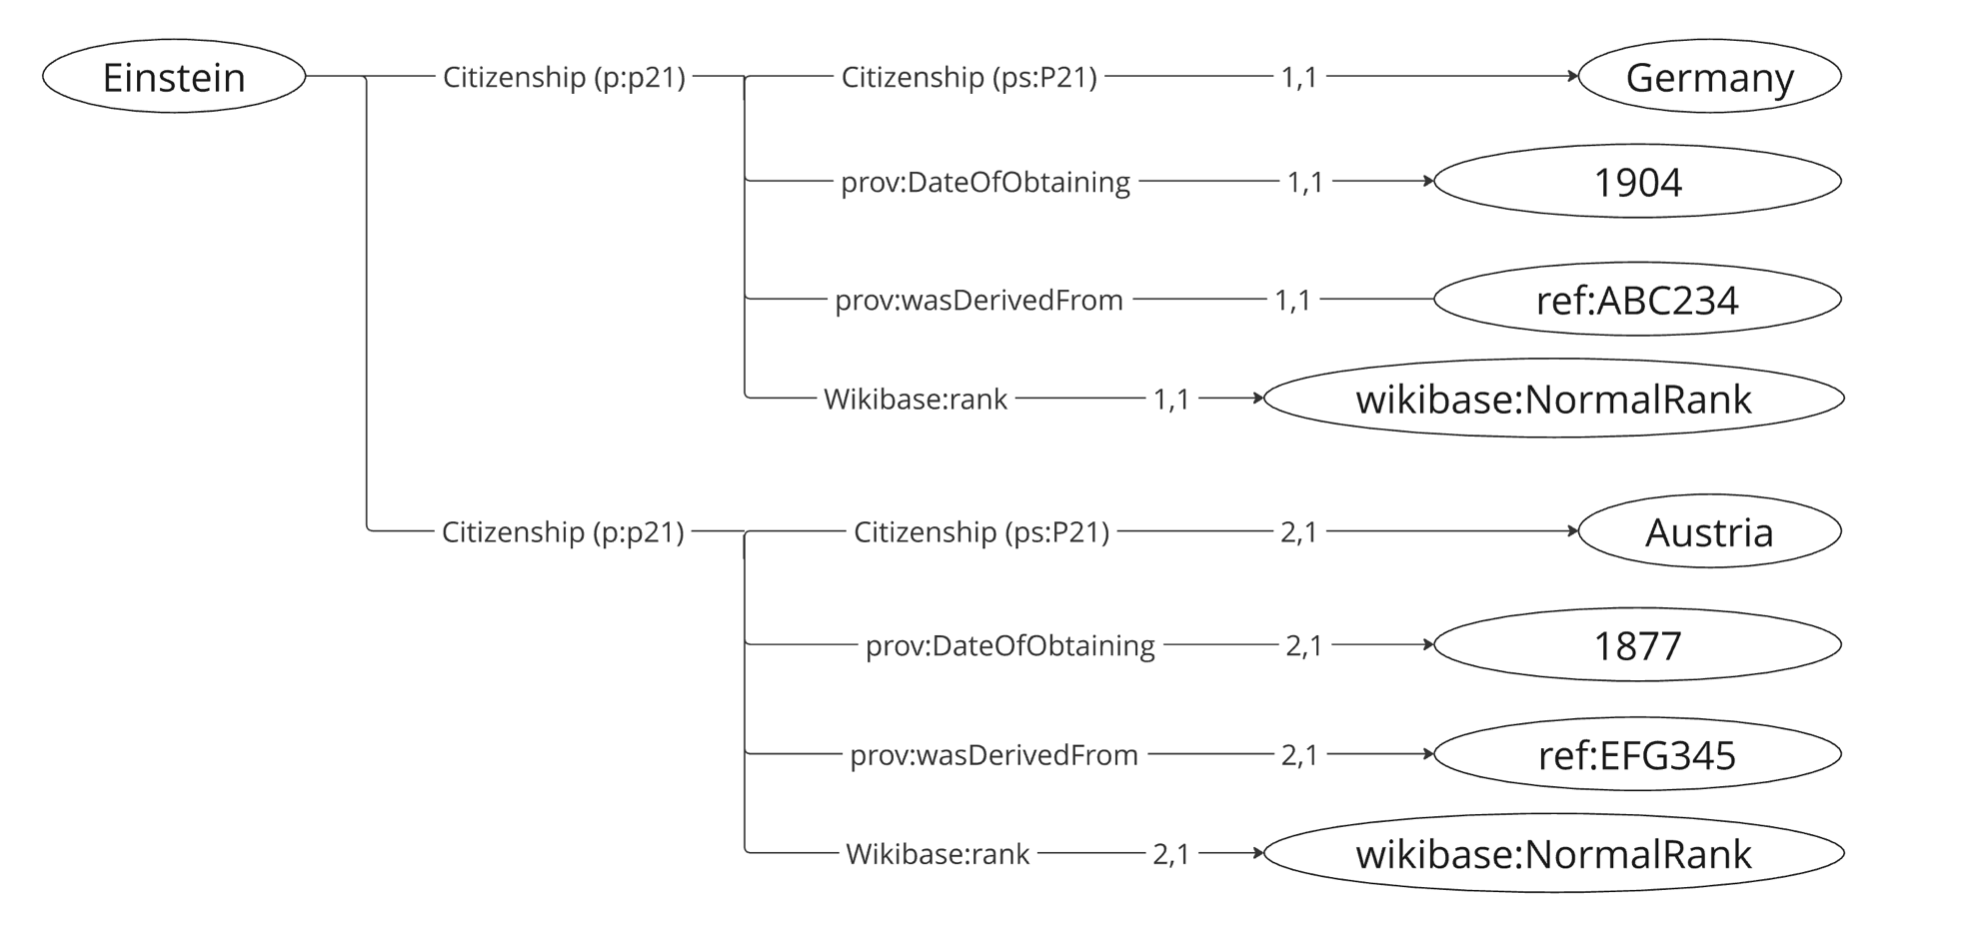
\includegraphics[width=0.8\textwidth]{13.png}
    \caption{New RDF Data Representation Approach}
    \label{fig:image13}
\end{figure}

The serialisation from the figure 13 in a new format can be presented in a code:

{\footnotesize
\begin{verbatim}
Einstein <p:P21|ps:P21>[1,1] Germany
Einstein <p:P21|pq:DateOfObtaining>[1,1] "1904"^^xsd:date
Einstein <p:P21|prov:wasDerivedFrom>[1,1] ref:ABC234
Einstein <p:P21|wikibase:rank>[1,1] wikibase:NormalRank

Einstein <p:P21|ps:P21>[2,1] Austria
Einstein <p:P21|pq:DateOfObtaining>[2,1] "1877"^^xsd:date
Einstein <p:P21|prov:wasDerivedFrom>[2,1] ref:EFG345
Einstein <p:P21|wikibase:rank>[2,1] wikibase:NormalRank
\end{verbatim}
}

Sometimes in Wikidata there are predicate chains, like <p:P21|ps:P21>. P (property) is a connector from a subject to a statemnt, and ps (property statement) is a connector of statement to an object. It is possible to merge p with ps:

{\footnotesize
Einstein <p:P21>[1,1] Germany
\end{verbatim}
}

\subsubsection{Indexing system}

To handle multiple values for the same predicate chain (like multiple citizenships), we introduce an indexing system. This system allows us to maintain order and differentiate between multiple instances:

{\footnotesize
\begin{verbatim}
wd:Q42 <p:P27|ps:P27>[1,1] wd:Q183
wd:Q42 <p:P27|ps:P27>[1,2] wd:Q40
wd:Q42 <p:P27|ps:P27>[1,3] wd:Q30
\end{verbatim}
}

In this example, Einstein's citizenships (German, Austrian, and American) are represented with distinct index values.

The first index represents the first predicate. If a subject has more than one similar predicate, like "married to", we enumerate each of the predicates to prevent the marriage problem. The next predicate in a chain (e.g., of statement, like reference, rank etc.) will be attached to the right predicate.

The last index represents the indexing of elements of the predicate, that touches object. It helps to enumerate elements, that have same predicates and subjects, that are written by "," in the other formats, like turtle. There is still a discussion, whether each object has to have his own line of code, or whether the objects can be written in one line.

{\footnotesize
\begin{verbatim}
wd:Q42 <p:P27|ps:P27>[1,1] wd:Q183
wd:Q42 <p:P27|ps:P27>[1,2] wd:Q40
wd:Q42 <p:P27|ps:P27>[1,3] wd:Q30
\end{verbatim}
}

Alternatively we can introduce a shorthanded format to make the new format more readable.

{\footnotesize
\begin{verbatim}
wd:Q42 <p:P27|ps:P27>[1,1:3] wd:Q183, wd:Q40, wd:Q30
\end{verbatim}
}

Or

{\footnotesize
\begin{verbatim}
wd:Q42 <p:P27|ps:P27>[1;1,2,3] wd:Q183, wd:Q40, wd:Q30
\end{verbatim}
}

The second solution is the shortest. We don't need to keep enumerated values, instead just a range, like in python. However, if an element will be removed from the list of values, then the problem starts. E.g, we remove the second element, would then the third element become the second? For now we decided to stick with the first – even though it takes a lot of space, it is easy to remove an element. The enumeration, however remains. The next added element will have an enumeration of max(n) + 1.

All the prefixes are written in the beginning and have the task of shortening the length of each element by aliasing IRI (Internationalized Resource Identifiers).

% For now, there are no considerations in adding special cases or extra functions to an algorithm.

The strength of this approach becomes evident when dealing with qualifiers and references. Instead of creating separate statement nodes, we extend the predicate chain and use multi-level indexing:

{\footnotesize
\begin{verbatim}
wd:Q42 <p:P27>[1] wd:Q183
wd:Q42 <p:P27|pq:P580>[1,1] "1904"^^xsd:date
wd:Q42 <p:P27|prov:wasDerivedFrom>[1,1] wdref:ABC234
wd:Q42 <p:P27|wikibase:rank>[1,1] wikibase:NormalRank
\end{verbatim}
}

This structure efficiently represents that Einstein's German citizenship was obtained in 1904, the information was derived from reference ABC234, and it has a normal rank in Wikidata.

\subsubsection{Advantages over RDF* and Traditional RDF}

The chained predicate approach we have developed offers several significant advantages over both RDF*. By eliminating the need for reification or nested triples, our method simplifies the overall data structure, making it more straightforward and easier to manage. This simplicity is particularly valuable when dealing with complex metadata structures common in large-scale knowledge bases like Wikidata.

One of the key benefits of our approach is its efficiency. By removing intermediary nodes, we substantially reduce the total number of triples required to represent complex statements. This reduction in data volume not only saves storage space but also potentially improves query performance by reducing the amount of data that needs to be processed.

% The indexed structure we've implemented allows for more direct and efficient querying of specific instances or qualifiers. This enhanced query ability is crucial for large-scale data management, where the ability to quickly retrieve specific pieces of information can significantly impact system performance and user experience.

Our format also offers greater flexibility compared to RDF* and traditional RDF. It can easily accommodate additional metadata without the need to introduce new structural elements. This adaptability is particularly valuable in evolving knowledge bases where new types of metadata or relationships may need to be incorporated over time.

Our approach effectively solves the "Marriage Problem" that has been a persistent issue with RDF*. Multiple instances of relationships can now be represented without ambiguity or redundancy, addressing one of the major limitations that motivated our research in the first place.

In essence, we have created an alternative solution to RDF* where the property table is replaced by a combination of <property-chain> and <cardinality-chain>. Our approach was directly motivated by the limitations we encountered with RDF*, particularly issues like the repeated marriage triples problem. By addressing these challenges, our method offers a more robust and efficient way of representing complex, metadata-rich RDF data, especially for large-scale knowledge bases like Wikidata.

    
\begin{figure}[htbp]
    \centering
    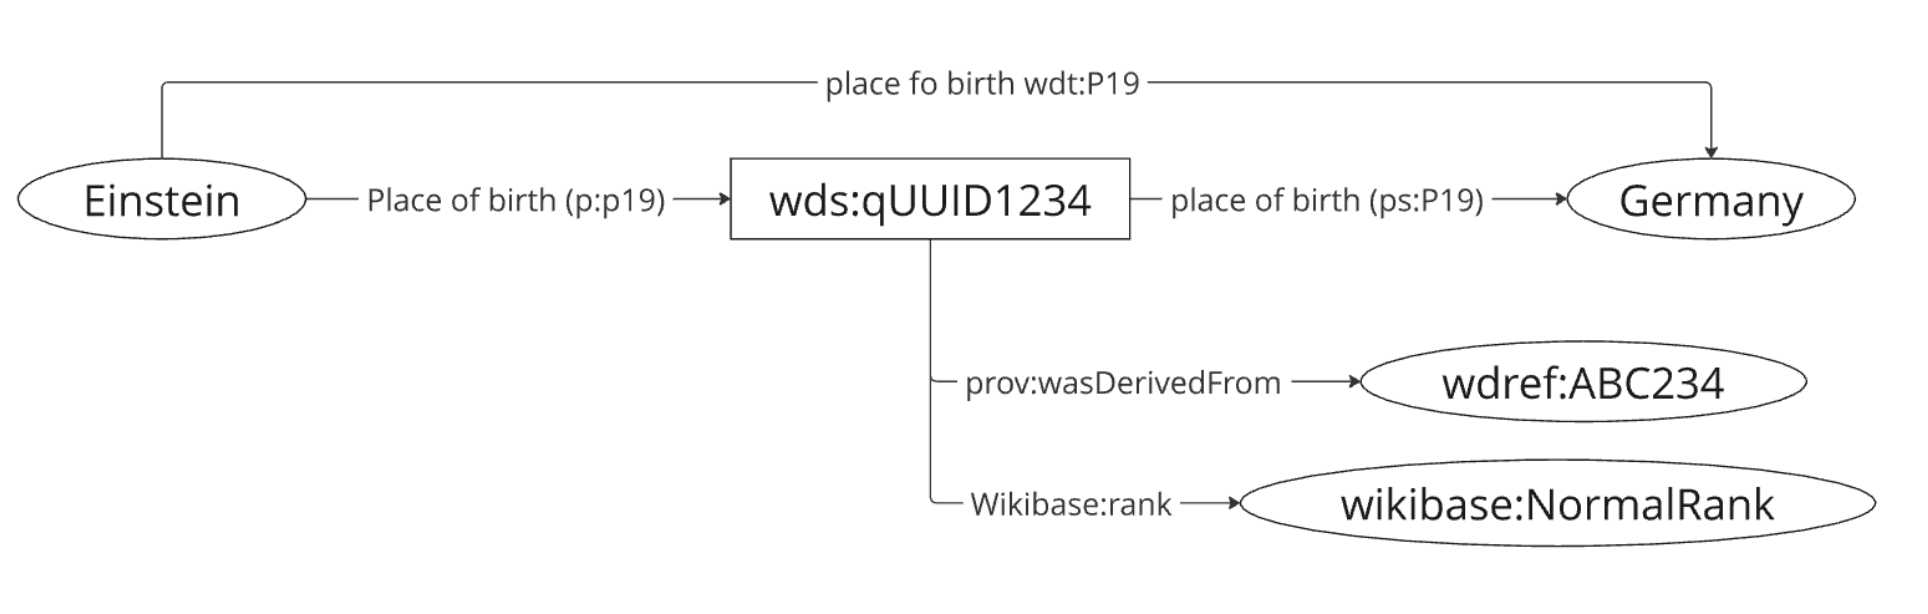
\includegraphics[width=0.8\textwidth]{14.png}
    \caption{Statement structure in Wikidata}
    \label{fig:image14}
\end{figure}

The Figure 14 illustrates the current structure of Wikidata in Turtle format. As we can see, there is a statement wds:qUUID1234 that acts as an intermediary node, holding three triples: place of birth, prov:wasDerivedFrom, and Wikibase:rank. Our new approach aims to simplify this structure.

Our new algorithm removes the intermediary statement between the main subject and object. Instead, this statement is transformed into a chain of predicates with indexation of the elements. This transformation eliminates nested statements, meaning every object now has equal status and carries meaningful information rather than just serving as a link to other objects.

\begin{figure}[htbp]
    \centering
    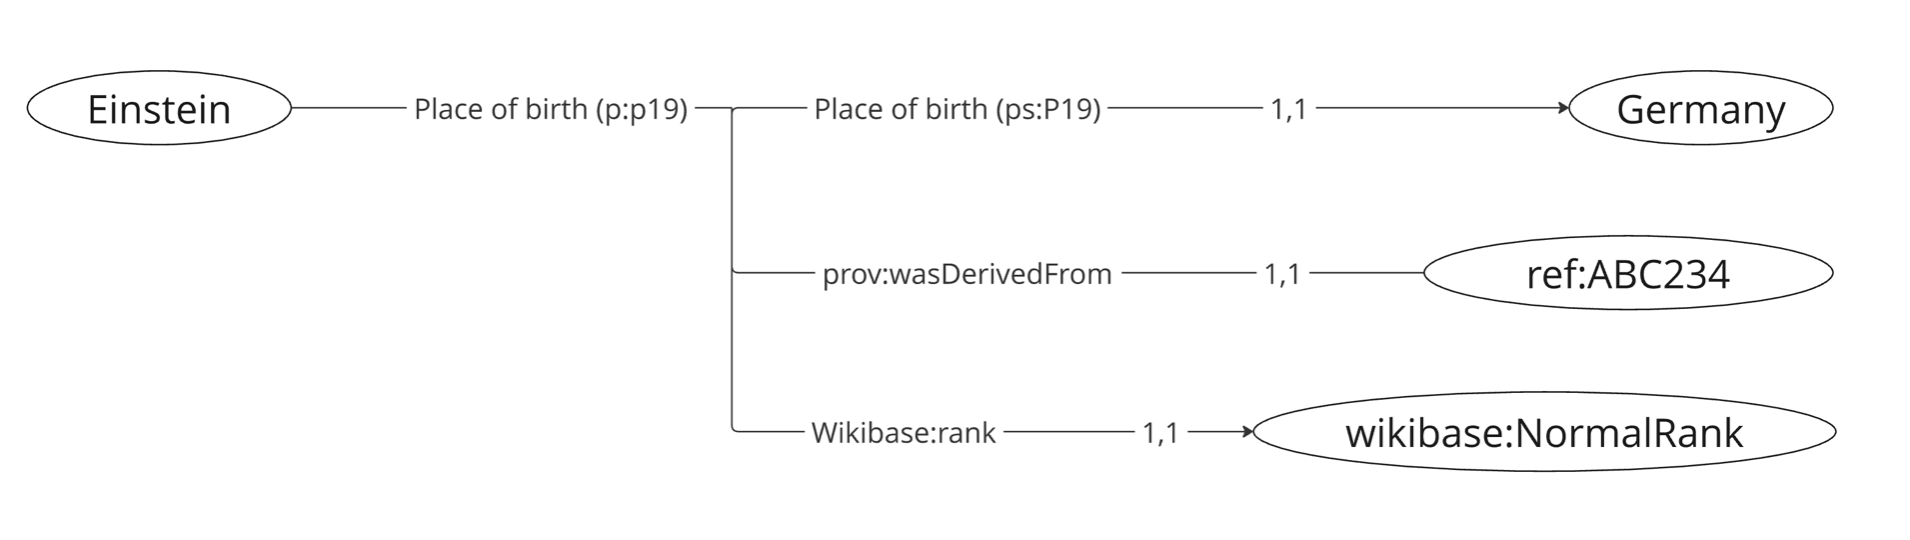
\includegraphics[width=0.8\textwidth]{15.png}
    \caption{New approach to statement structure in Wikidata}
    \label{fig:image15}
\end{figure}

In this new structure, we can represent the same information more efficiently. For example, Einstein's place of birth would be represented as:

{\footnotesize
\begin{verbatim}
Einstein <p:P19|ps:P19>[1,1] Germany
Einstein <p:P19|prov:wasDerivedFrom>[1,1] ref:ABC234
Einstein <p:P19|wikibase:rank>[1,1] wikibase:NormalRank
\end{verbatim}
}

This approach not only simplifies the data structure but also makes it more intuitive and easier to query. The chained predicates and indexed values allow for a clear representation of the relationships and metadata without the need for intermediary nodes or complex nested structures.

To better illustrate our approach, let's consider some examples. For instance, if Einstein has the identifier wd:Q42, a predicate p:P1, and an object wd:Q39, the statement in our new format would be written as:

{\footnotesize
\begin{verbatim}
wd:Q42 <p:P1>[1] wd:Q39
\end{verbatim}
}

If we add another predicate p:P2 with object wd:Q123, we would have:

{\footnotesize
\begin{verbatim}
wd:Q42 <p:P1>[1] wd:Q39
wd:Q42 <p:P2>[1] wd:Q123
\end{verbatim}
}

Our format also allows for multiple objects with the same predicate:

{\footnotesize
\begin{verbatim}
wd:Q42 <p:P1>[1] wd:Q39
wd:Q42 <p:P1>[2] wd:Q51
wd:Q42 <p:P2>[1] wd:Q123
\end{verbatim}
}

For more complex statements involving metadata, we use chains of predicates with multi-level indexing:

{\footnotesize
\begin{verbatim}
wd:Q42 <p:P19|a>[1,1] Wikibase:BestRank
wd:Q42 <p:P19|wd>[1,2] wd:Q123
wd:Q42 <p:P19|prov>[1,3] WasDerivedFrom ref:SOMEUUID5678
\end{verbatim}
}

This structure eliminates the need for extra statements. All information is written together, with the chain of predicates and indexation providing a clear hierarchy and relationship between elements.

In contrast to the current Wikidata format shown in the first image, where a statement (wds:qUUID1234) acts as an intermediary holding multiple triples, our new algorithm removes this intermediary. The statement is transformed into a chain of predicates with indexed elements. This approach eliminates nested statements, giving each object equal status and meaningful content rather than just serving as links to other objects.

This representation not only simplifies the data structure but also makes it more intuitive and easier to query, addressing the limitations we identified in traditional RDF and RDF* formats.

\subsubsection{Predicate chain and indexing}

\begin{figure}[htbp]
    \centering
    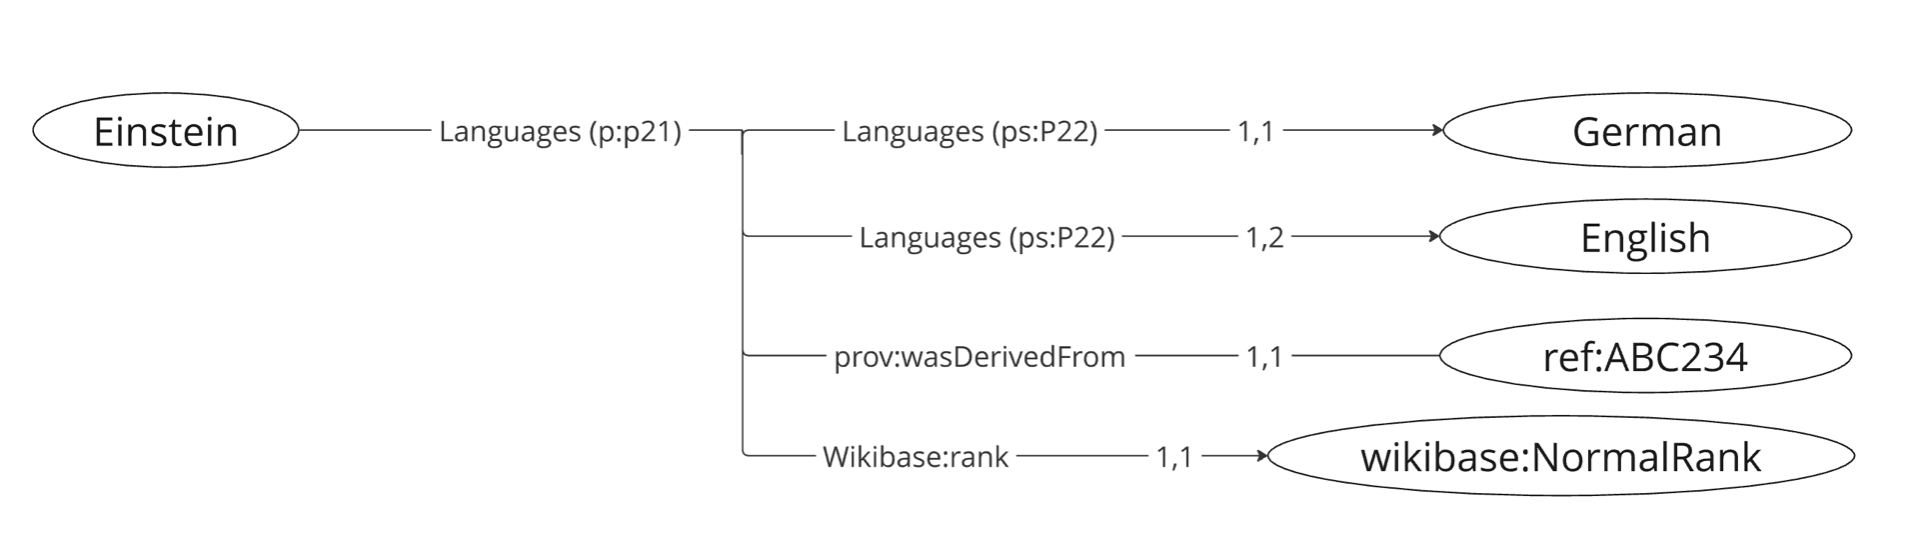
\includegraphics[width=1\textwidth]{16.png}
    \caption{New approach to statement structure in Wikidata}
    \label{fig:image16}
\end{figure}

The predicate chain collects all predicates that connect the subject to the object. These predicates are written in a format of <first-predicate|second-predicate>, for example <p:P27|ps:P27>. By using this approach, we eliminate unnecessary nested statements and maintain only subjects and objects, simplifying the overall structure while preserving semantic relationships.

However, using just a predicate chain is not enough. If there are multiple values, like citizenships, we want to keep track on which country of citizenship are we interested in. In the given example, the citizenships are Germany and Austria (obtained in different time, dates are not accurate and chosen for demonstration purposes)

\begin{figure}[htbp]
    \centering
    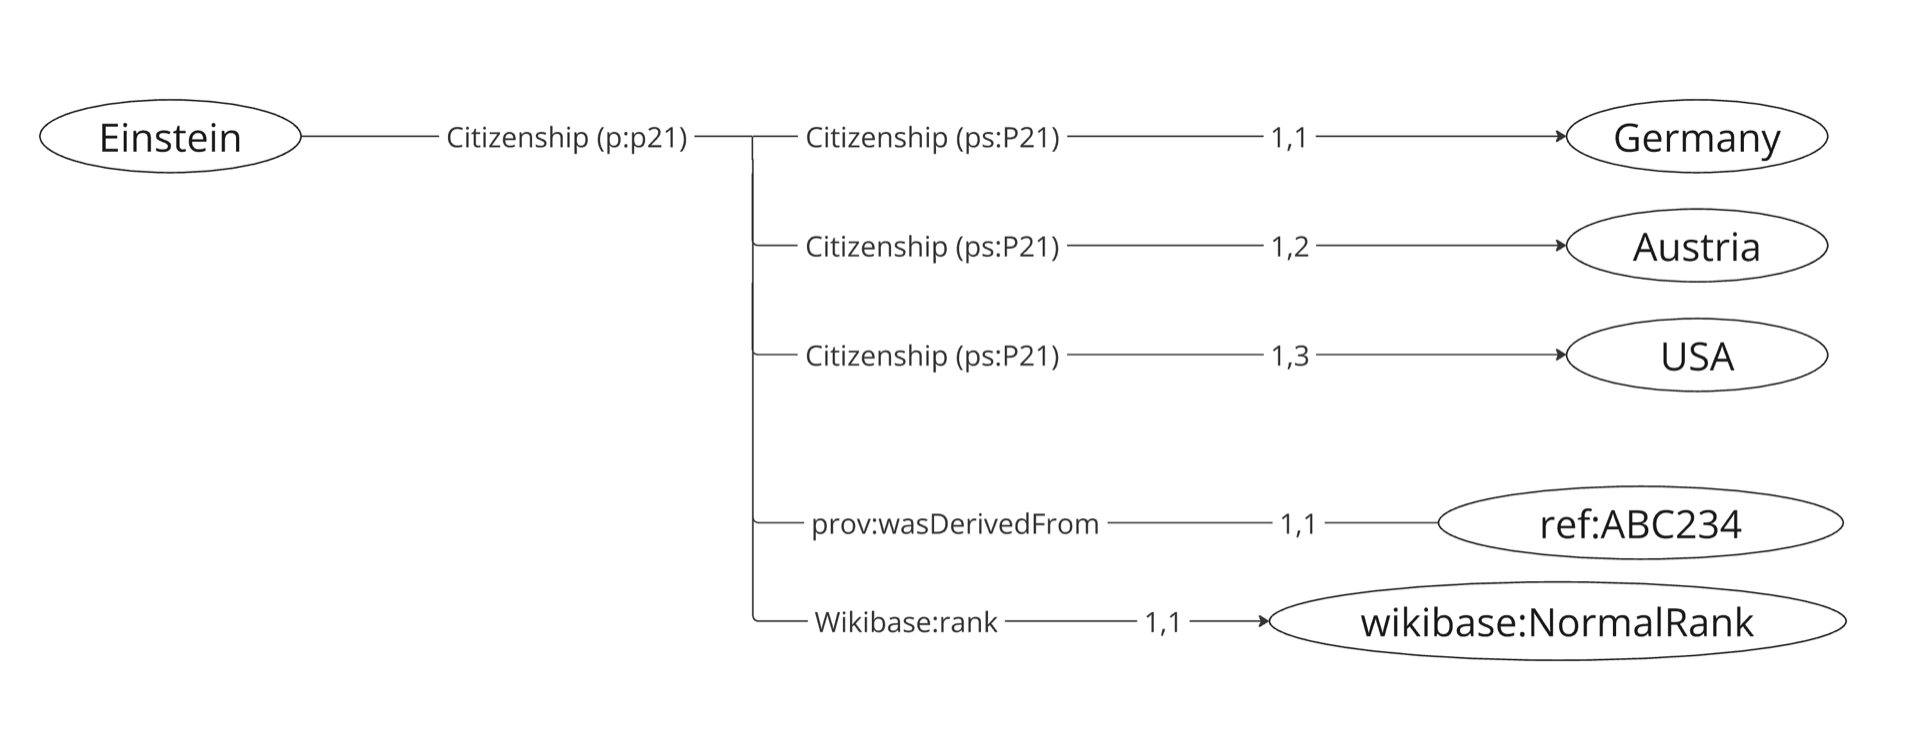
\includegraphics[width=1\textwidth]{17.png}
    \caption{New approach to statement structure in Wikidata with multiple values (example only for the first value, second has its own chain of predicates and indexation)}
    \label{fig:image17}
\end{figure}

{\footnotesize
\begin{verbatim}
Einstein <p:P21|ps:P21>[1,1] Germany
Einstein <p:P21|ps:P21>[1,2] Austria
Einstein <p:P21|ps:P21>[1,3] USA
\end{verbatim}
}

The indexes [1,1], [1,2], and [1,3] differentiate between the three citizenship statements, that makes simple the processing of attaching information or metadata about each statements, as shown in the image:

{\footnotesize
\begin{verbatim}
Einstein <p:P21|prov:wasDerivedFrom>[1,1] ref:ABC234
Einstein <p:P21|wikibase:rank>[1,1] wikibase:NormalRank
\end{verbatim}
}

The predicates are extracted from the existing Turtle format using a custom script that analyzes the structure of each statement. This script identifies the hierarchy of predicates and constructs the appropriate chains.

% The syntax of this approach is similar RDF. Each statement consistently has a subject in the first position, a predicate (or chain of predicates with indexes) in the second position, and objects in the third position. Theoretically, these triples could be entered into a table with 3 columns: subjects, predicates, and objects using querying. The finding of elements becomes then closer to the SQL format, even though it's not entirely accurate to draw a direct comparison.

The syntax of this approach is similar to RDF. Each statement consistently has a subject in the first position, a predicate in the second position, and objects in the third position. When a chain of predicates is used, each predicate is assigned a unique index to maintain order. Theoretically, these triples could be entered into a table with separate columns for subjects, predicates, indexes, and objects using querying. The finding of elements becomes then closer to the SQL format, even though it’s not entirely accurate to draw a direct comparison.
\section{Implementation}

The implementation is not focused on the speed of the program and has a main purpose of understanding how much space does the same file require for a new format comparing with Turtle format. It is important for a research to also see how special situations, like statement on statement are simplified using the given approach.

\subsection{Wikidata specifics}
Wikidata has nearly 140Gb of data as described before. It has different prefixes, some of which include:

{\footnotesize
\begin{verbatim}
@prefix cc: <http://creativecommons.org/ns#> .
@prefix data: <https://www.wikidata.org/wiki/Special:EntityData/> .
@prefix owl: <http://www.w3.org/2002/07/owl#> .
@prefix p: <http://www.wikidata.org/prop/> .
@prefix pq: <http://www.wikidata.org/prop/qualifier/> .
@prefix pqn: <http://www.wikidata.org/prop/qualifier/value-normalized/> .
@prefix pqv: <http://www.wikidata.org/prop/qualifier/value/> .
@prefix pr: <http://www.wikidata.org/prop/reference/> .
@prefix prn: <http://www.wikidata.org/prop/reference/value-normalized/> .
@prefix prov: <http://www.w3.org/ns/prov#> .
@prefix prv: <http://www.wikidata.org/prop/reference/value/> .
@prefix ps: <http://www.wikidata.org/prop/statement/> .
@prefix psn: <http://www.wikidata.org/prop/statement/value-normalized/> .
@prefix psv: <http://www.wikidata.org/prop/statement/value/> .
@prefix rdfs: <http://www.w3.org/2000/01/rdf-schema#> .
@prefix ref: <http://www.wikidata.org/reference/> .
@prefix s: <http://www.wikidata.org/entity/statement/> .
@prefix schema1: <http://schema.org/> .
@prefix skos: <http://www.w3.org/2004/02/skos/core#> .
@prefix v: <http://www.wikidata.org/value/> .
\end{verbatim}
}

In this list, there are prefixes that define statement values (psv), reference values (prv and prov), and qualifier values (pqv – similar to statements, they contain multiple triples defining some values):

{\footnotesize
\begin{verbatim}
s:Q937-33ce60f7-4629-0ab4-38d9-701633f118da
    (some triples here)
    pqv:P580 v:a8cb14e3f795be35aa7849c41cac676a ;

v:a8cb14e3f795be35aa7849c41cac676a a wikibase:TimeValue ;
    wikibase:timeCalendarModel wd:Q1985727 ;
    wikibase:timePrecision 9 ;
    wikibase:timeTimezone 0 ;
    wikibase:timeValue "1908-01-01T00:00:00+00:00"^^xsd:dateTime .

s:Q937-DA60BC41-F680-461A-A3A7-9D675CEEF2B8 a wikibase:BestRank,
        wikibase:Statement ;
    wikibase:rank wikibase:NormalRank ;
    ps:P2021 2.0 ;
    psv:P2021 v:45430454bd0f3bc0d9093c52b6acfc2b .

v:45430454bd0f3bc0d9093c52b6acfc2b a wikibase:QuantityValue ;
    wikibase:quantityAmount 2.0 ;
    wikibase:quantityUnit wd:Q199 .
\end{verbatim}
}

These prefixes of predicates are referring to another statements. That means, they become a part of a chain of predicates. The prefixes of objects are also indicating reference to statements: s (statement), ref (reference), and v (value).
% When the prefixes are found, the predicate chain will be created. For this, a recursive function will be used.

\subsection{The Software and Hardware}
To convert Turtle to the new format, I use a Python script. The program does not require specific libraries beyond the standard library. For the experiment, I use a MacBook Pro with 8Gb of RAM, 50gb of free disk space, and an M1 processor. Currently, I don't have access to more powerful hardware, which limits the conversion of the full Wikidata dataset (with the chosen algorithm). The Wikidata file is too large for the available disk space, and the processor would require a substantial amount of time due to the algorithm's complexity. Therefore, a small chunk of 1 megabyte will be used in this research. The primary goal is to convert the data, not to optimize for speed. It's anticipated that such transformation would occur infrequently (in the case of Wikidata, every time a new dump is released, approximately once a month).

I use Python 3.12, which provides all the necessary features for the given tasks. To facilitate the transformation process, I have set up a local server using FastAPI that accepts text and .txt documents as input. As output, it returns a .txt file in the new format specified earlier. While the program runs locally, it can also be deployed to the cloud, for example, on a server at the Vienna University of Economics and Business.

\subsection{Code implementation}
\begin{figure}[htbp]
    \centering
    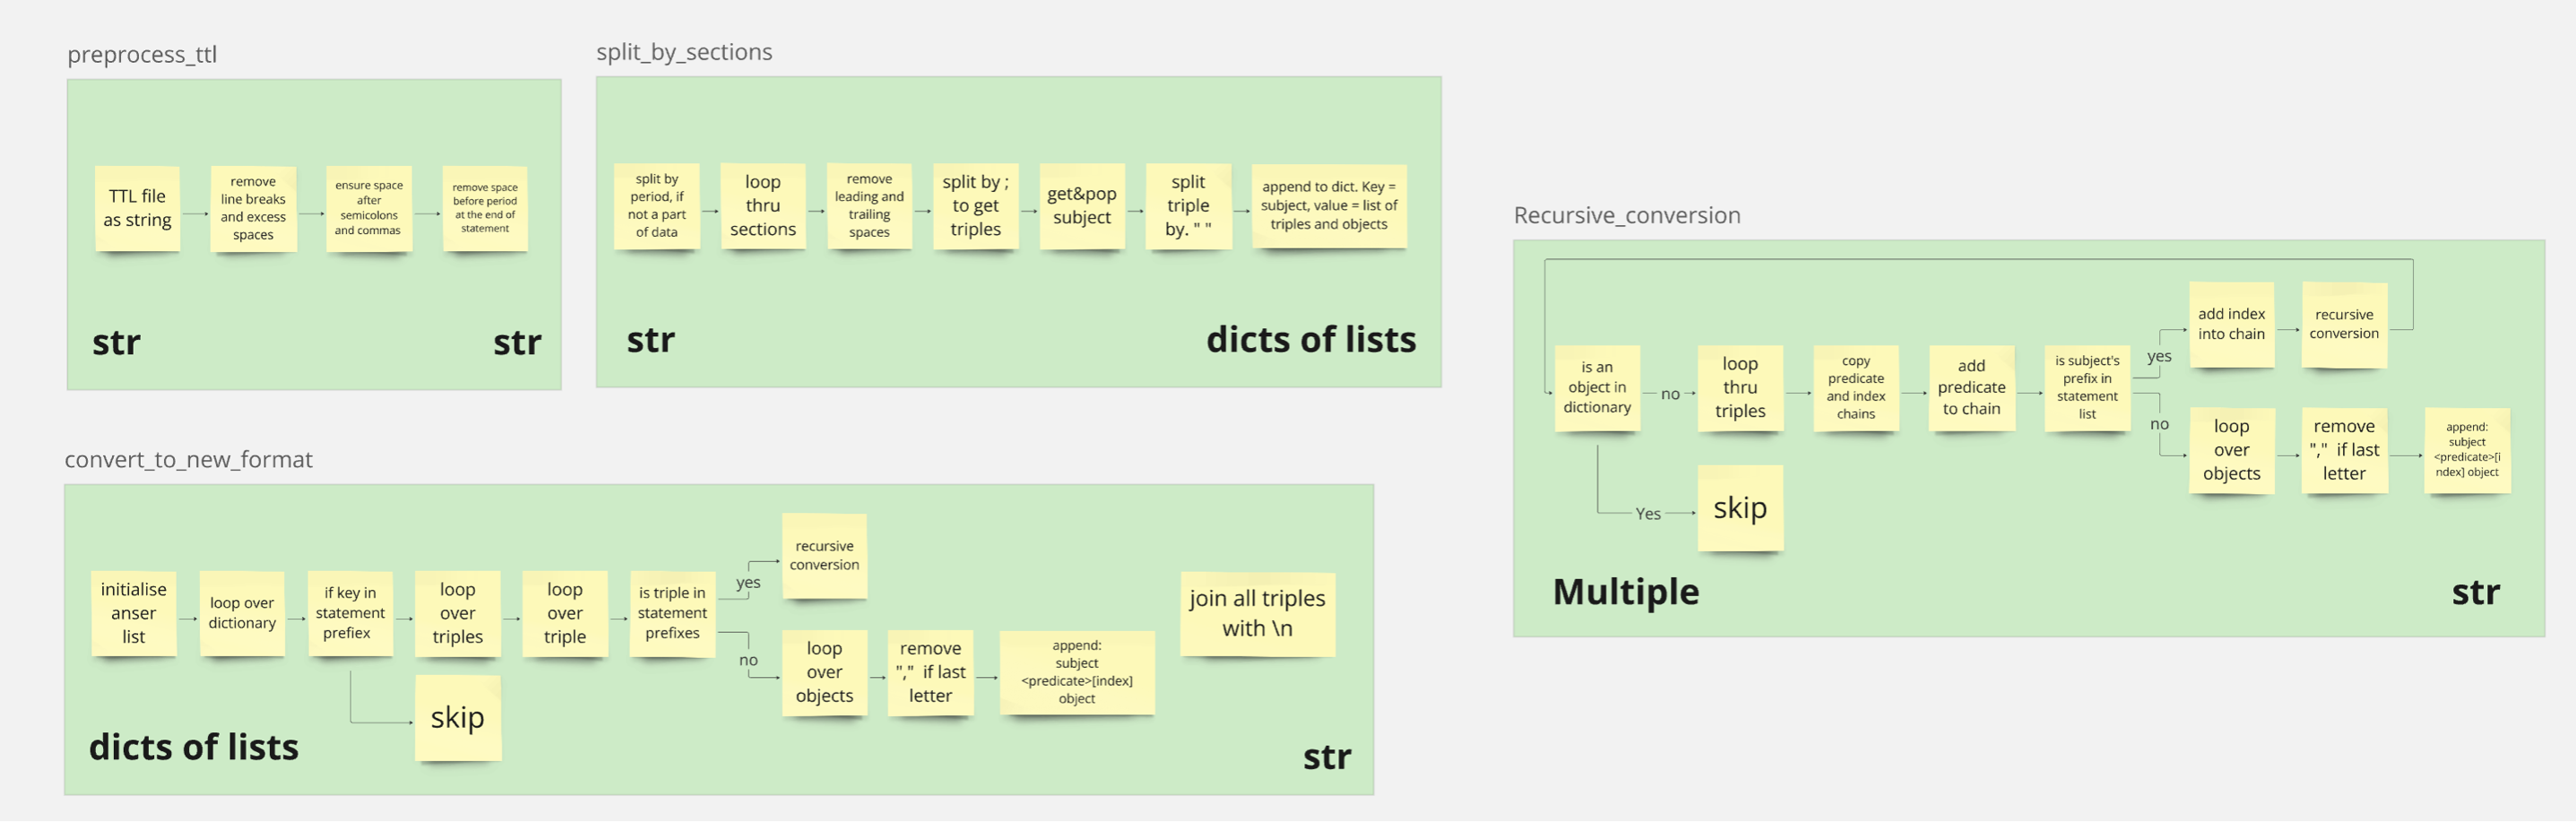
\includegraphics[width=1\textwidth]{18.png}
    \caption{Converting Turtle to the new format.}
    \label{fig:image18}
\end{figure}

The code is written in Python and is available on GitHub at \url{https://github.com/Koveh/ttl-converter}. The current version converts Turtle to the new format. It can process most of the Turtle syntax, including prefixes, blank nodes represented as lists of predicates and objects, and statements with one subject and multiple predicates and objects, as well as multiple objects for one predicate. However, it currently cannot store blank nodes that lack a parent statement, and it cannot handle values that are not associated with any subjects.


The algorithm is divided into Preprocessing and Conversion parts. In the preprocessing stage, the initial Turtle text is enhanced, prefixes are extracted and stored separately, and the text is split into statements, triples, and elements of triples. The result is a dictionary with subjects as keys and the rest of the statements as values, represented as lists of triples, each containing a list of elements.

Another part of preprocessing involves identifying blank nodes, which are presented in statements as lists of predicates and objects. These are then represented as qualified statements with a subject in the form of a random UUID and added to the dictionary of statements. The rationale for this approach is explained in the following sections.

The Conversion part transforms the dictionary into the new format, writing the result line by line to a new text file. The dictionary is processed step by step. Each triple is analyzed for qualified statements as objects. When found, a recursive function processes the qualified statement, extracting all predicates and objects and incorporating them into the triple of the initial subject. If a qualified statement contains another qualified statement, the same recursive function is applied.

The final output is a text file with prefixes at the top followed by the triples. The resulting format is straightforward and doesn't use any special operators like lists, indentation, or references to other objects.

Let's now examine each function to explain the transformation process in detail. Note that while some functions could be implemented more simply, the constraints of the Turtle format and the need for additional conversions, such as handling blank nodes (which were not initially planned), increased the complexity. The code is open-source, and contributions are welcome.

\subsubsection{Imports and constants}
The current code requires two libraries: re for the regex and uuid for generating unique identifiers for the blank nodes. Afterwards, the statement prefixes are defined. After a manual search, I have found that Wikidata uses s:, v:, ref: for qualified statements and references, which are signals to the hierarchy of predicate chains. The blank node prefix is added by me and is used together with the generated uuid.

Two libraries, 'time' and 'typing' are optional. They are used for performance measurement (counting of amount needed to make preprocessing and conversion parts) and type hinting, respectively.

{\footnotesize
\begin{verbatim}
import re
from typing import Dict, List, Tuple
import uuid
import time

# Statement prefixes used to identify special statements in the Turtle format
STATEMENT_PREFIX = ["s:", "v:", "ref:", "blank-node:"]
\end{verbatim}
}

\subsubsection{Preprocessing}
The preprocessing function is divided into multiple parts: removing unnecessary whitespace, extracting prefixes, splitting the text into statements, triples, and elements of triples. It takes a string as input and returns a dictionary of statements, where each statement is a list of triples, and each triple is a list of elements.

This data structure is chosen to facilitate the search for qualified statements. The nested list structure allows for easy conversion of triples. While it would be possible to process the file line by line to reduce memory usage, especially for large datasets like Wikidata, the current approach prioritizes processing speed over memory efficiency.

Storing statements in a dictionary with subjects as keys enables fast lookups. Python dictionaries use hash tables, resulting in O(1) search complexity, which means search speed remains constant regardless of the dictionary's size. This approach is particularly efficient when dealing with large volumes of qualified statements.

The 'preprocess\_ttl' function uses regular expressions to normalize whitespace, ensure proper spacing around punctuation, and handle periods correctly. While the regex implementation is unconventional, it allows for a single pass through the text instead of multiple passes for each normalization stage.

{\footnotesize
\begin{verbatim}
def preprocess_ttl(ttl_text: str) -> str:
    """
    Preprocesses a TTL (Turtle) text by normalizing whitespace and punctuation.
    """
    # Use regex to normalize whitespace and ensure proper spacing around punctuation
    preprocessed = re.sub(
        r'\s+|([;,])(?!\s)|(?<=[^;\s])\s*\.',
        lambda m: ' ' if m.group(0).isspace() else f'{m.group(1)} ' if m.group(1) else '.',
        ttl_text
    )
    # Remove trailing spaces and periods
    return preprocessed.rstrip(' .')
\end{verbatim}
}

The next three functions split the text by periods, semicolons, and spaces while preserving quoted content. This is necessary because literal objects may contain punctuation that should not be used for splitting. For example, the regex pattern \verb|r';\s*(?=(?:[^"]"[^"]")[^"]$)'| matches semicolons followed by spaces, ensuring that semicolons inside quotes are not matched.

{\footnotesize
\begin{verbatim}
def split_by_periods_keep_quotes(text: str) -> List[str]:
    """
    Split the text by periods, but keep quoted content intact.
    """
    pattern = r'\\.\s+(?=(?:[^"]*"[^"]*")*[^"]*$)'
    sections = re.split(pattern, text)
    return [section.strip() for section in sections]

def split_by_semicolons_keep_quotes(text: str) -> List[str]:
    """
    Split the text by semicolons, but keep quoted content intact.
    """
    pattern = r';\s*(?=(?:[^"]*"[^"]*")*[^"]*$)'
    statements = re.split(pattern, text)
    return [statement.strip() for statement in statements]

def split_by_spaces_keep_quotes(text: str) -> List[str]:
    """
    Split the text by spaces, but keep quoted content and URIs intact.
    """
    pattern = r'"(?:\\.|[^"\\])*"[^\s]*|"(?:\\.|[^"\\])*"|[^\s"]+'
    return re.findall(pattern, text)
\end{verbatim}
}

\subsubsection{Bracket processing}
This function handles brackets enclosing blank nodes. Initially, it assumed blank nodes couldn't be nested, but it was later updated to handle nested blank nodes. The function uses a stack-based approach similar to solving the "Polish notation problem" to keep track of opening and closing brackets. It recursively processes the text, handling nested brackets. Each created statement is assigned a subject with the prefix "blank-node:" followed by a UUID. This subject is an intermediary used during processing and doesn't appear in the final format. The original blank node in the Turtle format is replaced with this new subject.

{\footnotesize
\begin{verbatim}
def check_for_brackets(section: str, dictionary_of_sections: Dict[str, List[List[str]]]) -> str:
    """
    Process a section of text, replacing bracketed content with UUIDs.
    """
    def process_brackets(text: str, start: int) -> Tuple[str, int]:
        """
        Find the matching closing bracket for an opening bracket.
        """
        stack = 1
        end = start + 1
        while stack > 0 and end < len(text):
            if text[end] == '[':
                stack += 1
            elif text[end] == ']':
                stack -= 1
            end += 1
        return text[start + 1:end - 1].strip(), end

    def recursive_process(text: str) -> str:
        """
        Recursively process the text, handling nested brackets.
        """
        while '[' in text:
            start = text.find('[')
            content, end = process_brackets(text, start)
            processed_content = recursive_process(content)
            new_uuid = f"blank-node:{uuid.uuid4()}"
            statements = split_by_semicolons_keep_quotes(processed_content)
            dictionary_of_sections[new_uuid] = [split_by_spaces_keep_quotes(statement) for statement in statements]
            text = text[:start] + new_uuid + text[end:]
        return text

    return recursive_process(section)
\end{verbatim}
}

\subsubsection{Section splitting}
This function combines all the above functions. It takes as input the string of the Turtle file and the dictionary of sections, processing the entire input to produce the structured representation used in the conversion stage.

{\footnotesize
\begin{verbatim}
def split_by_sections(preprocessed_text: str, dictionary_of_sections: Dict[str, List[List[str]]]) -> Tuple[Dict[str, List[List[str]]], str]:
    """
    Split the text into sections by periods.
    """
    sections = split_by_periods_keep_quotes(preprocessed_text)
    result = {}
    prefixes = []

    for section in sections:
        if section.startswith("@prefix"):
            prefixes.append(section + ' .')
        else:
            section = check_for_brackets(section, dictionary_of_sections)
            stripped_section = section.strip()
            statements = split_by_semicolons_keep_quotes(stripped_section)
            subject = statements[0].split(" ")[0]
            statements[0] = statements[0].replace(subject + " ", "")
            result[subject] = [split_by_spaces_keep_quotes(statement) for statement in statements]

    return result, "\n".join(prefixes)
\end{verbatim}
}

\subsubsection{Conversion}
The main function here is 'convert\_and\_write\_to\_file', which takes our dictionary of sections and an output file as parameters. This function is complex due to the need to handle nested structures, so we've implemented a recursive approach.

Inside 'convert\_and\_write\_to\_file', we define a nested function called 'recursive\_conversion'. This function is crucial for dealing with qualified statements and nested structures. It takes predicate chains, index chains, objects, and subjects as parameters. The function checks if an object is actually a subject of another statement (indicating a qualified statement), and if so, it dives deeper into that statement, building up the predicate and index chains as it goes.

The main loop of 'convert\_and\_write\_to\_file' iterates through our sections dictionary. For each subject and its triples, it checks if the subject is a special statement (starting with our defined prefixes) and skips it if so. Then, for each triple, it either calls the recursive function for qualified statements or writes a simple statement to the output file.

One tricky part was handling the indexes correctly. We need to keep track of the position of each predicate and object in the original data structure, which is why we build up these index chains. This ensures that our new format accurately represents the structure of the original data.

{\footnotesize
\begin{verbatim}
def convert_and_write_to_file(sections: Dict[str, List[List[str]]], output_file):
    """
    Convert sections to the required format and write to file.
    """
    def recursive_conversion(predicate_chain, index_chain, object, subject):
        """
        Recursively convert nested structures and write to file.
        """
        if object not in sections:
            return

        for triple in sections[object]:
            if not triple:
                print(f"Warning: Empty triple found for object {object}")
                continue

            new_predicate_chain = predicate_chain + [triple[0]]

            if len(triple) > 1 and triple[1].startswith(tuple(STATEMENT_PREFIX)) and object != triple[1]:
                for i, obj in enumerate(triple[1:], start=1):
                    obj = obj[:-1] if obj.endswith(',') else obj
                    new_index = index_chain + [str(i)]
                    recursive_conversion(new_predicate_chain, new_index, obj, subject)
            else:
                predicates = "|".join(new_predicate_chain)
                for i, obj in enumerate(triple[1:], start=1):
                    obj = obj[:-1] if obj.endswith(',') else obj
                    new_index = index_chain + [str(i)]
                    indexes = ",".join(new_index)
                    output_file.write(f'{subject} <{predicates}>[{indexes}] {obj}\n')

    for subject, triples in sections.items():
        if subject.startswith(tuple(STATEMENT_PREFIX)):
            continue
        for triple in triples:
            if not triple:
                print(f"Warning: Empty triple found for subject {subject}")
                continue

            predicate_chain = [triple[0]]

            for i, obj in enumerate(triple[1:], start=1):
                obj = obj[:-1] if obj.endswith(',')

                if len(triple) > 1 and triple[1].startswith(tuple(STATEMENT_PREFIX)) and triple[1] != subject:
                    recursive_conversion(predicate_chain, [str(i)], obj, subject)
                else:
                    predicate = triple[0]
                    output_file.write(f'{subject} <{predicate}>[{i}] {obj}\n')
\end{verbatim}
}

\subsubsection{Main function}
The main function serves as the orchestrator of our entire process. It's responsible for reading the input file, calling our preprocessing and conversion functions, and writing the output. We've also included some timing functions to measure the performance of our preprocessing and conversion steps separately.

First, we attempt to read the input Turtle file. We've wrapped this in a try-except block to handle the case where the file isn't found, providing a user-friendly error message. Then, we initialize our dictionary of sections and call our preprocessing functions.

After preprocessing, we merge our main sections dictionary with the dictionary of sections that came from processing blank nodes. This ensures all our data is in one place for the conversion step.

We've added timing measurements around both the preprocessing and conversion steps. This gives us valuable information about which part of our process might be a bottleneck, especially when dealing with large files.

Finally, we write our output, starting with the prefixes we extracted earlier, followed by our converted data. Again, we've used a try-except block here to handle potential write errors gracefully.

{\footnotesize
\begin{verbatim}
def main():
    """
    Main function to read input, process TTL, and write output.
    """
    try:
        with open('einstein.ttl', 'r', encoding='utf-8') as input_file:
            ttl_text = input_file.read()
    except FileNotFoundError:
        print("Input file not found.")
        return

    dictionary_of_sections = {}

    start_time = time.time()
    preprocessed_ttl = preprocess_ttl(ttl_text)
    sections, prefixes = split_by_sections(preprocessed_ttl, dictionary_of_sections)
    sections.update(dictionary_of_sections)
    end_time = time.time()
    print(f"Preprocessing executed in {end_time - start_time} seconds.")

    start_time = time.time()
    try:
        with open('output.txt', 'w', encoding='utf-8') as output_file:
            output_file.write(prefixes + "\n")
            convert_and_write_to_file(sections, output_file)
    except IOError as e:
        print(f"Error writing to output file: {e}")
        return
    end_time = time.time()
    print(f"Conversion executed in {end_time - start_time} seconds.")
\end{verbatim}
}

One challenge we faced was balancing memory usage with processing speed. Reading the entire file into memory at once might not be feasible for very large Turtle files. In future versions, we might consider implementing a streaming approach to handle arbitrarily large inputs without running out of memory.

\subsubsection{Transformation into HDT format}
The new approach is not ideal due to frequent repeatings of subjects, as well as predicates, that are repreating themselves in every qualified statement. Implementing HDT into a new structure will save space. The conversion process is similar to the conversion of RDF to HDT: subjects and objects are put into dictionaries to either S, O or SO table and are provided with unique identifier. The difference comes in conversion of indexes and predicate chains into the dictionary. The predicate chains are also repeating on the large amount of data, therefore predicate chains can also be stored in the dictionary section. The question is whehter the predicate chains have to be stored in the predicate section of a dictionary or in a new dictionary section, where each predicate chain is presented in a form of a list of unique identifiers of predicates. 

The indexes should be stored in a triple section. Even though, that most index are [1] and [1,1], there are a lot of unique indexes, like [1,1,5,2]. Storing of them in the dictionary is unnecessary and it makes more difficult Querying the data due to unnecessary search in an index dictionary. But, to prove whether indexes have to be stored in the dictionary or be written in the triple section, the experiments have to be made.

\section{Evaluation and Results}

The algorithm was tested on a 1Mb dataset about Einstein, comprising 31.5k lines (24,077 without blank lines) of Turtle data. This sample size is sufficient to verify correct data conversion and assess the readability of the new format. The einstein.ttl file (available on GitHub at \url{https://github.com/Koveh/ttl-converter}) included all necessary Turtle elements, such as prefixes, literal objects, blank nodes, statements, and triples in statements that share the same object and subject. The research was conducted on a personal computer as described in the previous section.

The code transformed 31.5k lines (24,077 without blank lines) to 24,057 lines, which appears to be a minor difference. However, the new file size is 1,344,189 bytes, compared to 1,035,723 bytes in the original Turtle format, representing a 30\% increase. Extrapolating this to the full Wikidata dataset would result in a file size of approximately 200Gb.


\subsection{RDF format comparison}
The RDF format of the same Einstein dataset has 40280 lines, or 2.8Mb, which is more than 2 times larger, than the new format. Turtle file was converted using RDFlib library on python to the RDF format.

The new format in example with Wikidata, when compared to traditional RDF, presents a significant departure from the nested structure typically associated with RDF representations. Instead of utilizing an XML-like format with nested elements, this novel approach employs predicate chains and indexing to represent hierarchical relationships, similar to SQL database or csv with 4 columns: subject, predicate chain, index and object. This structure offers several advantages in terms of data representation and accessibility. Below, i compared a simple triple of a the new format with traditional Turtle and RDF/XML respectively:

{\footnotesize
\begin{verbatim}
wd:P1430 <rdfs:label>[1] "Open Plaques subject ID"@en

wd:P1430 a wikibase:Property ;
    rdfs:label "Open Plaques subject ID"@en ;

<rdf:Description rdf:about="http://www.wikidata.org/entity/P1430">
    <rdfs:label xml:lang="en">Open Plaques subject ID</rdfs:label>
</rdf:Description>
\end{verbatim}
}

The new format eliminates the need to traverse multiple levels of nesting to understand the relationship between entities. It may lead to more efficient data processing and querying, as the hierarchical structure is encoded directly in the predicate chain and index.

\subsection{HDT format comparison}
To save space, we can convert the new format to HDT-like format, where each subject, object, predicate will be stored in a Dictionary and will have a short Unique identifier. On the table below there is an amount of unique values in each table. The last column represets amount of bits required to store unique identifiers for this amount of values.

% \begin{table}[htbp]
%     \centering
%     \begin{tabular}{|c|c|c|}
%         \hline
%         \textbf{Column Index} & \textbf{Unique Count} & \textbf{Bits Required} \\
%         \hline
%         Subjects & 6602 & 13 \\
%         Predicate chains & 2607 & 12 \\
%         Indexes & 405 & 9 \\
%         Objects & 8347 & 13 \\
%         \hline
%     \end{tabular}
%     \caption{Column statistics}
%     \label{tab:column_stats}
% \end{table}


\begin{table}[htbp]
    \centering
    \begin{tabular}{|l|r|r|r|r|}
        \hline
        \textbf{Metric} & \textbf{TTL} & \textbf{RDF} & \textbf{HDT} & \textbf{New Format} \\
        \hline
        File Size & 1,035,723 bytes & 2,800,000 bytes & 286,700 bytes & 1,344,189 bytes \\
        Number of Lines & 24,077 & 40,280 & N/A & 24,057 \\
        Number of Triples & 24,492 & 24,492 & 24,492 & 24,057 \\
        Different Subjects & 7,882 & 7,882 & 7,882 & 6,602 \\
        Different Predicates & 1,409 & 1,409 & 1,409 & 2,607 \\
        Different Objects & 10,060 & 10,060 & 10,060 & 8,347 \\
        \hline
    \end{tabular}
    \caption{Comparison of Different Data Formats}
    \label{tab:comparison_table}
\end{table}

As we may observe, predicate chains may have two thousand unique values, while the total amount of triples is more than 24 thousand. Indexes are also repeating themselves, but they are short and usually have only one number, therefore, it is possible to write them directly in the triple section of HDT.

To understand whether this amount is suitable, I compared HDT dictionary and triples with the new format. First, I converted TTL to RDF and then converted RDF to HDT using official rdfhdt program on Java, that can be found on Github.

% \begin{table}[htbp]
%     \centering
%     \begin{tabular}{|l|r|}
%         \hline
%         \textbf{Metric} & \textbf{Value} \\
%         \hline
%         Original Size & 3.1Mb \\
%         HDT Size & 286.7 KB \\
%         Compression Ratio & 9.13\% \\
%         \hline
%     \end{tabular}
%     \caption{Dataset Statistics}
%     \label{tab:dataset_stats}
% \end{table}

% \begin{table}[htbp]
%     \centering
%     \begin{tabular}{|l|r|}
%         \hline
%         \textbf{Metric} & \textbf{Value} \\
%         \hline
%         Number of Entries & 12,222 \\
%         Different Subjects & 7,882 \\
%         Different Predicates & 1,409 \\
%         Different Objects & 10,060 \\
%         Shared Area & 7,129 \\
%         Dictionary Size & 206.7 KB \\
%         \hline
%     \end{tabular}
%     \caption{Dictionary Statistics}
%     \label{tab:dictionary_stats}
% \end{table}

% \begin{table}[htbp]
%     \centering
%     \begin{tabular}{|l|r|}
%         \hline
%         \textbf{Metric} & \textbf{Value} \\
%         \hline
%         Number of Triples & 24,492 \\
%         Triples Size & 132.1 KB \\
%         \hline
%     \end{tabular}
%     \caption{Triples Statistics}
%     \label{tab:triples_stats}
% \end{table}

% \begin{table}[htbp]
%     \centering
%     \begin{tabular}{|l|r|}
%         \hline
%         \textbf{Metric} & \textbf{Value} \\
%         \hline
%         Number of Triples & 24,492 \\
%         Different Subjects & 7,882 \\
%         Different Predicates & 1,409 \\
%         Different Objects & 10,060 \\
%         \hline
%     \end{tabular}
%     \caption{Vanilla RDF Statistics. Turtle has exactly same amount}
%     \label{tab:vanilla_rdf_stats}
% \end{table}

The number of subjects in the new format is reduced by approximately 1,000 compared to the original format, and the amount of objects in the new format is approximately 1,700 lower than in the original format, which is a positive indicator. This reduction suggests that the new format is more efficient in handling repetitive data, particularly in large-scale datasets like Wikidata.

The use of HDT saved 90 percent of space (from 2.8Mb to 286.7Kb), therefore, the conversion of a new format to the HDT-like format is a good idea.

% The amount of predicates in HDT is smaller than predicate chains in the new format. Possibly, it is better to store predicates in dictionary instead of predicate chains, and store predicate chains in the triples section. In the triple section, the predicates will occupy more space and will be written as predicate chain. Usage of the bitmap may help to save space when the chain contains similar predicate in the beginning.

The amount of predicates in HDT is smaller than predicate chains in the new format. Possibly, it is better to store predicate chains in the dictionary instead of individual predicates, as these chains will repeat many times in large datasets. In the triple section, we would then only need to store compact indexes. Usage of bit operations may help to save space when representing these indexes in the triple section.

\subsection{Time}

Preprocessing took 1.9 seconds, while conversion took 0.016 seconds. The use of a dictionary format for statements, which enables O(1) key lookup using hash tables, prevented the recursive algorithm from becoming overly complex when finding required statements.

The majority of processing time was spent on preprocessing, which involves numerous constraints such as handling blank nodes, literal nodes containing elements like ".", ";", "," inside brackets, and "$\wedge\wedge$", "@en" etc. outside. This necessitates regex checking for every triple. Additionally, converting each line from Turtle to a suitable format, where each element becomes a string in a list of lists in a dictionary with the subject as the key, contributes to the lengthy preprocessing time.

While time efficiency is not the primary focus of this research, it's worth considering the time required to convert larger datasets. Given the use of dictionaries with O(1) complexity, the number of elements should not significantly impact performance.

Extrapolating the results: 1 gigabyte of data would require approximately 1,900 seconds for preprocessing and 16 seconds for conversion. 140 gigabytes would take about 75 hours (1,916 * 140 / 3600). This speed is already suitable for processing Wikidata. The algorithm could potentially be optimized further through multiprocessing techniques.

\subsection{Readability}

Let's take a look at the following conversion. The entity wd:Q937 (Einstein) has 61,303 triples. Some are straightforward, like:

{\footnotesize
\begin{verbatim}
wd:Q937 wdt:P6385[1] "nauka_i_tehnika/fizika/ENSHTEN_ALBERT.html"
\end{verbatim}
}

where wdt:P6385 represents "Vikipedia article title-lat". Others are more complex and contain lists of different values.

{\footnotesize
\begin{verbatim}
wd:Q937 <rdfs:label>[43] "Эйнштейн Альберт"@cv
wd:Q937 <rdfs:label>[44] "Albert Einstein"@cy
wd:Q937 <rdfs:label>[45] "Albert Einstein"@da
wd:Q937 <rdfs:label>[46] "Albert Einstein"@dag
wd:Q937 <rdfs:label>[47] "Albert Einstein"@de
wd:Q937 <rdfs:label>[48] "Albert Einstein"@de-at
wd:Q937 <rdfs:label>[49] "Albert Einstein"@de-ch
\end{verbatim}
}

Other are more complex and include "statements".

{\footnotesize
\begin{verbatim}
wd:Q937 <p:P7502|a>[1,1] wikibase:BestRank
wd:Q937 <p:P7502|a>[1,2] wikibase:Statement
wd:Q937 <p:P7502|wikibase:rank>[1,1] wikibase:NormalRank
wd:Q937 <p:P7502|prov:wasDerivedFrom|a>[1,1,1] wikibase:Reference
wd:Q937 <p:P7502|prov:wasDerivedFrom|pr:P813>[1,1,1] "2022-09-10T00:00:00+00:00"^^xsd:dateTime
wd:Q937 <p:P7502|prov:wasDerivedFrom|pr:P854>[1,1,1] <https://golden.com/wiki/Albert_Einstein-N6Y>
wd:Q937 <p:P7502|prov:wasDerivedFrom|prv:P813|a>[1,1,1,1] wikibase:TimeValue
wd:Q937 <p:P7502|prov:wasDerivedFrom|prv:P813|wikibase:timeCalendarModel>[1,1,1,1] wd:Q1985727
wd:Q937 <p:P7502|prov:wasDerivedFrom|prv:P813|wikibase:timePrecision>[1,1,1,1] 11
wd:Q937 <p:P7502|prov:wasDerivedFrom|prv:P813|wikibase:timeTimezone>[1,1,1,1] 0
wd:Q937 <p:P7502|prov:wasDerivedFrom|prv:P813|wikibase:timeValue>[1,1,1,1] "2022-09-10T00:00:00+00:00"^^xsd:dateTime
wd:Q937 <p:P7502|ps:P7502>[1,1] "Albert_Einstein-N6Y"
\end{verbatim}
}

Some are even more complex, including the multiple qualitative statements for one predicate.

{\footnotesize
\begin{verbatim}
wd:Q937 <p:P27|a>[5,1] wikibase:BestRank
wd:Q937 <p:P27|a>[5,2] wikibase:Statement
wd:Q937 <p:P27|wikibase:rank>[5,1] wikibase:NormalRank
wd:Q937 <p:P27|prov:wasDerivedFrom|a>[5,1,1] wikibase:Reference
wd:Q937 <p:P27|prov:wasDerivedFrom|pr:P854>[5,1,1] <https://newspapers.ushmm.org/events/albert-einstein-quits-germany-renounces-citizenship>
wd:Q937 <p:P27|prov:wasDerivedFrom|a>[5,2,1] wikibase:Reference
wd:Q937 <p:P27|prov:wasDerivedFrom|pr:P227>[5,2,1] "118529579"
wd:Q937 <p:P27|prov:wasDerivedFrom|pr:P248>[5,2,1] wd:Q23833686
wd:Q937 <p:P27|prov:wasDerivedFrom|pr:P813>[5,2,1] "2024-05-03T00:00:00+00:00"^^xsd:dateTime
wd:Q937 <p:P27|prov:wasDerivedFrom|prn:P227>[5,2,1] <https://d-nb.info/gnd/118529579>
wd:Q937 <p:P27|prov:wasDerivedFrom|prv:P813|a>[5,2,1,1] wikibase:TimeValue
wd:Q937 <p:P27|prov:wasDerivedFrom|prv:P813|wikibase:timeCalendarModel>[5,2,1,1] wd:Q1985727
wd:Q937 <p:P27|prov:wasDerivedFrom|prv:P813|wikibase:timePrecision>[5,2,1,1] 11
wd:Q937 <p:P27|prov:wasDerivedFrom|prv:P813|wikibase:timeTimezone>[5,2,1,1] 0
wd:Q937 <p:P27|prov:wasDerivedFrom|prv:P813|wikibase:timeValue>[5,2,1,1] "2024-05-03T00:00:00+00:00"^^xsd:dateTime
\end{verbatim}
}

The code is readable and understandable. The new format maintains a clear structure that allows for easy interpretation of the data hierarchy. Each line represents a single piece of information, with the subject (wd:Q937) consistently at the beginning, followed by the predicate chain enclosed in angle brackets, and then the object. The index values in square brackets provide a clear indication of the statement's position within the overall structure. Even without the qualitative statements, the format is clear both for humans, and machines.

% \subsection{Potential issue}

% One issue, that also remains in other formats is a removal of a triple that has child triples. In such cases, all child triples must also be removed to maintain data integrity. To identify child triples, we can search for triples with matching predicate chains and indexes, plus an additional predicate and index. For example:

% Parent triple:
% {\footnotesize
% \begin{verbatim}
% wd:Q937 <p:P27|prov:wasDerivedFrom|prn:P227>[5,2,1] https://d-nb.info/gnd/118529579
% \end{verbatim}
% }

% Child triples:
% {\footnotesize
% \begin{verbatim}
% wd:Q937 <p:P27|prov:wasDerivedFrom|prv:P813|a>[5,2,1,1] wikibase:TimeValue
% wd:Q937 <p:P27|prov:wasDerivedFrom|prv:P813|wikibase:timeCalendarModel>[5,2,1,1] wd:Q1985727
% wd:Q937 <p:P27|prov:wasDerivedFrom|prv:P813|wikibase:timePrecision>[5,2,1,1] 11
% \end{verbatim}
% }

% The child triples have a similar chain, with the only difference being that they have n+1 predicates and n+1 indexes. Implementing a cascading delete operation would be necessary to maintain consistency.





\section{Future Work and Potential Improvements}

As this research project concludes, we identified several approaches for future work and potential improvements. These enhancements can boost efficiency and applicability of the new format for managing large-scale RDF data, particularly in the context of Wikidata.

For more qualified research, more tests and benchmarks have to be performed to ensure that the new method is more efficient than vanilla HDT, TTL or RDF format. The disadvantage of the current research is in an inability to use large datasets, like Wikidata. This is due to lack of computational resources. The new format should be tested and compared on the large variety of datasets, to ensure the storage efficiency of the algorithm.

Optimisation of an algorithm and rewriting it in C++ may make the converter faster than the existing approaches for other rdf structures, like rdf2hdt. Even though the speed of conversion is not an important parameter, because in the real world the conversion is done once. Optimisation is more important here. One of the problems of the current approach is that the whole text file of the code has to be kept in memory in a form of dictionary. Processing the data in memory necessitates RAM capacity at least equivalent to the size of the input file.

The implementation of HDT conversion of a new approach is another important milestone. Structure of the new HDT format is crucial. Series of tests of various structures of a new HDT format have to be performed. As discussed before, we have to decide to either keep predicates or predicate chains in the dictionary, or a separate dictionary for predicates with their UUID combinations in predicate chain dictionary. The structure of triples and and whether to compress triples using bitmap technology to save space are another themes for discussion.

These potential improvements and directions for future work highlight the dynamic nature of research in RDF data management. As we continue to push the boundaries of what's possible with linked data and knowledge graphs, ongoing refinement and optimization of our approaches will be crucial in handling the ever-growing scale and complexity of datasets like Wikidata.

\bibliographystyle{apacite}
\bibliography{reference}

\end{document}
